%%%%%%%%%%%%%%%%%%%%%%%%%%%%%%%%%%%%%%%%%%%%%%%%%%%%%%%%%%%%%%%%%%%%%%%%%%%%%
%%%
%%% File: thesis.tex, version 1.9, May 2016
%%%
%%% =============================================
%%% This file contains a template that can be used with the package
%%% cs.sty and LaTeX2e to produce a thesis that meets the requirements
%%% of the Computer Science Department from the Technical University of Cluj-Napoca
%%%%%%%%%%%%%%%%%%%%%%%%%%%%%%%%%%%%%%%%%%%%%%%%%%%%%%%%%%%%%%%%%%%%%%%%%%%%%

\documentclass[12pt,a4paper,twoside]{report}  
\usepackage{hyperref}
\usepackage{cs}
%\usepackage[options ]{algorithm2e}
\usepackage{multicol}
\usepackage{times}
\usepackage{graphicx}
\usepackage{latexsym}
\usepackage{amsmath,amsbsy}
\usepackage{amssymb}
\usepackage[matrix,arrow]{xy}
\usepackage[T1]{fontenc}
\usepackage[super]{nth}
\usepackage{comment}
\usepackage{ae,aecompl}
%\usepackage[romanian]{babel}
\usepackage{float}
\usepackage{romanian}
\usepackage{amstext}
\usepackage{graphics}
\usepackage[T1]{fontenc}
\usepackage{ae,aecompl}
\usepackage{relsize}
\usepackage{combelow}
\usepackage[linesnumbered,ruled,vlined]{algorithm2e}
%\usepackage{algorithmic}
\usepackage{listings}
\usepackage[table, svgnames, usenames, dvipsnames]{xcolor}
\DeclareMathOperator{\Rr}{\mathbb{R}^{mxn}}
\DeclareMathOperator{\Rrr}{\mathbb{R}^{n}}
\DeclareMathOperator{\Rplus}{\mathbb{R}^{+}}
\diplomathesis
% \leftchapter
\centerchapter
% \rightchapter
\singlespace
% \oneandhalfspace
% \doublespace
%\useshorthands{'}
%\defineshorthand{'s}{\cb{s}}
%\defineshorthand{'t}{\cb{t}}
%\defineshorthand{'S}{\cb{S}}
%\defineshorthand{'T}{\cb{T}}
%\useshorthands{`}
%\defineshorthand{`i}{\^{i}}
%\defineshorthand{`I}{\^{I}}
%\defineshorthand{`a}{\^{a}}
%\defineshorthand{`A}{\^{A}}


\lstdefinestyle{basePython}{
  language=Python,
  emptylines=1,
  breaklines=true,
  basicstyle=\ttfamily\color{black},
  moredelim=**[is][\color{blue}]{@}{@},
  moredelim=**[is][\color{red}]{&}{&},
  moredelim=**[is][\color{green}]{?}{?},
}

\renewcommand{\thesisauthor}{Andrei-Alexandru TULBURE}    %% Your name.
\renewcommand{\thesismonth}{July}     %% Your month of graduation.
\renewcommand{\thesisyear}{2019}      %% Your year of graduation.
\renewcommand{\thesistitle}{Component housing defect detection using convolutional neural networks} % Title
\renewcommand{\thesissupervisor}{Prof. dr. ing. Eva DULF}
\newcommand{\department}{FACULTY OF AUTOMATION AND COMPUTER SCIENCE\\
AUTOMATION DEPARTMENT}
\newcommand{\thesis}{DIPLOMA THESIS}
\newcommand{\uline}[1]{\rule[0pt]{#1}{0.4pt}}
\newcommand{\utcnlogo}{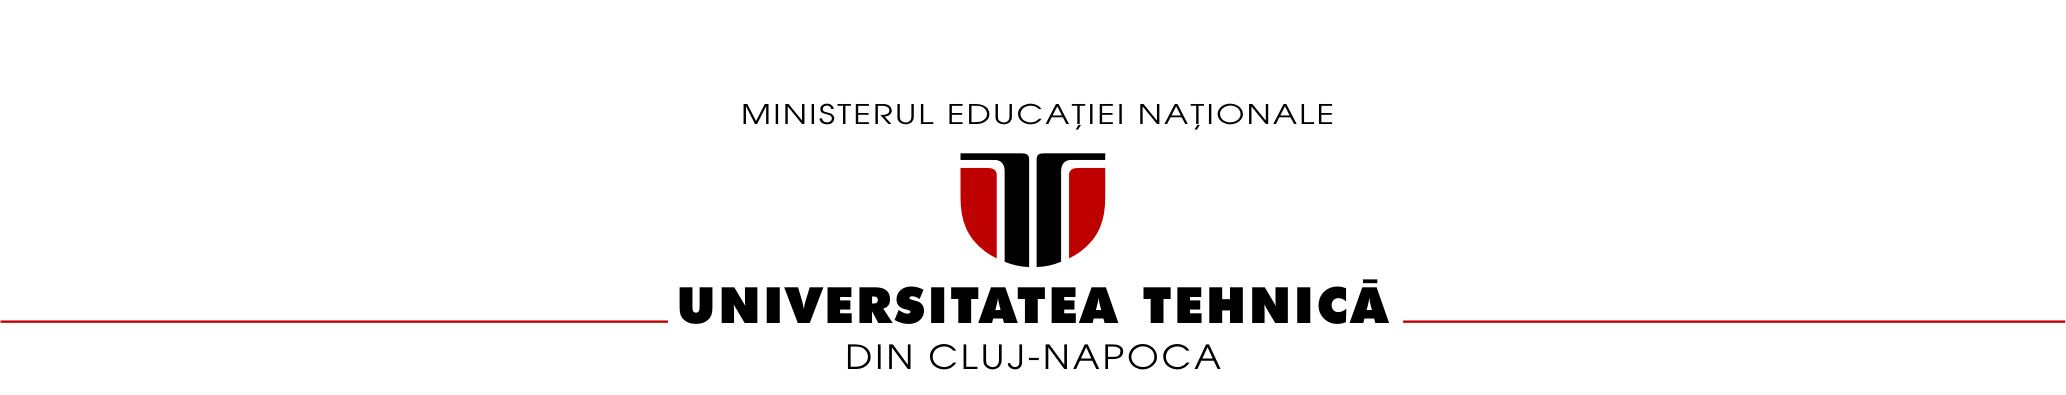
\includegraphics[width=15cm]{img/utcn.jpg}}


\begin{document}
%\frontmatter
%\pagestyle{headings}

\newenvironment{definition}[1][Defini'tie.]{\begin{trivlist}
\item[\hskip \labelsep {\bfseries #1}]}{\end{trivlist}}

%\thesistitle                    %% Generate the title page.
%\authordeclarationpage                %% Generate the declaration page.

\begin{center}

%\includegraphics[width=15cm]{img/tucn.jpg}  

\utcnlogo

{\bf \department}

\vspace{4cm}

{\bf \thesistitle} %LICENSE THESIS TITLE}

\vspace{1.5cm}

\thesis

\vspace{5cm}

Student: {\bf \thesisauthor} 

Scientific supervisor: {\bf \thesissupervisor}

\vspace{3cm}
{\bf \thesisyear}
\end{center}

\thispagestyle{empty}
\newpage

\begin{center}
\utcnlogo

{\bf \department}
\end{center}
\vspace{0.5cm}

%\begin{small}
\begin{tabular}{p{6cm}p{8cm}}
 %\hspace{-1cm}& VIZAT,\\
 \hspace{-1cm}DEAN, & DEPARTAMENT LEAD,\\
\hspace{-1cm}{\bf Prof. dr. ing. Liviu MICLEA} & {\bf Prof. dr. ing. Honoriu V'ALEAN}\\  
\end{tabular}
 
\vspace{1cm}

\begin{center}
Student: {\bf \thesisauthor}

\vspace{1cm}

{\bf \thesistitle}
\end{center}

\vspace{5mm}

\begin{enumerate}
 \item {\bf Title:} {\it The study and development of an artificial intelligence based solution for component housing defects detection using convolutional neural networks.}
\item {\bf Contents:} {\it Summary, Declaration, Table of content, Introduction, Project's purpose, Related work, Theoretical background, Design and implementation, Convolutional neural networks, Testing and validation, User guide for installation and use, Conclusions, Bibliography}
\item {\bf Development place:}  Technical University of Cluj-Napoca, Department of Automation
\item {\bf Consultants:} Prof. dr. ing. Eva DULF, Mr. Hari Polu, Mr. Lucian Man , Mr. Rodolfo Cruz.
\item {\bf Project start date:} 3 October 2018
\item {\bf Project end date:} 12 July 2019
  \end{enumerate}
\vspace{1.2cm}

\hspace{6cm} Student: \uline{6cm} 

\vspace{0.5cm}

\hspace{6cm} Scientific supervisor: \uline{5cm} 
%\end{small}

\thispagestyle{empty}


$ $
%\begin{center}
%\utcnlogo

%{\bf \department}
%\end{center}

\thispagestyle{empty}
\newpage

\begin{center}
\utcnlogo

{\bf \department}
\end{center}

\vspace{0.5cm}

\begin{center}
{\bf
Declara'tie pe proprie r'aspundere privind\\ 
autenticitatea lucr'arii de licen't'a}
\end{center}
\vspace{1cm}



Subsemnatul 
 \textbf{Andrei-Alexandru TULBURE}
legitimat cu \textbf{CI/BI} seria \textbf{AX} nr. \textbf{}, CNP \textbf{}, autorul lucr'arii \textbf{"Component housing defect detection using convolutional neural networks"}
elaborat'a 'in vederea sus'tinerii examenului de finalizare a studiilor de licen't'a la Facultatea de Automatic'a 'si Calculatoare, Specializarea        \textbf{Automatic'a} din cadrul Universit'a'tii Tehnice din Cluj-Napoca, sesiunea \textbf{iulie} a anului universitar \textbf{2018-2019}, declar pe proprie r'aspundere, c'a aceast'a lucrare este rezultatul propriei activit'a'ti intelectuale, pe baza cercet'arilor mele 'si pe baza informa'tiilor ob'tinute din surse care au fost citate, 'in textul lucr'arii 'si 'in bibliografie.

Declar, c'a aceast'a lucrare nu con'tine por'tiuni plagiate, iar sursele bibliografice au fost folosite cu respectarea legisla'tiei rom\ia ne 'si a conven'tiilor interna'tionale privind drepturile de autor.

Declar, de asemenea, c'a aceast'a lucrare nu a mai fost prezentat'a 'in fa'ta unei alte comisii de examen de licen't'a.

'In cazul constat'arii ulterioare a unor declara'tii false, voi suporta sanc'tiunile administrative, respectiv, \emph{anularea examenului de licen't'a}.

\vspace{1.5cm}

Data \hspace{8cm} Andrei-Alexandru, Tulbure

\vspace{0.5cm}

\uline{3cm} \hspace{5cm} \uline{5cm}

\vspace{1cm}
\hspace{9.4cm}Semn'atura

\thispagestyle{empty}

\begin{center}
\utcnlogo
\\
{\bf \department}
\begin{center}
\vspace{3mm}
\textbf{Synthesis}\\
of the diploma thesis:
\end{center}

\vspace{1mm}

{\bf \thesistitle}
\vspace{0.5cm}


\end{center}
Student: {\bf \thesisauthor}
\vspace{3mm}\\
\hspace{6cm} Scientific supervisor: \textbf{Prof. Dr. Ing. Eva DULF}
\vspace{1mm}\\
\begin{enumerate}
\item {\bf Thesis requirements:} To study the manufacturing process that needs to be automated proposed by OKOS Solutions USA. To study the available literature in the domain of computer vision. To study the theoretical background of Convolutional Neural Networks. To implement a CNN that is capable of classifying images fast and with high accuracy.
\item {\bf Chosen solutions:} In order to be able to detect defects I chose to implement a CNN-based algorithm, that returns if the component housing is has or has not defects. The images are provided partly by OKOS Solutions USA, partly enhanced by myself. The chosen architecture is a very deep CNN architecture called VGGNet developed at the Univ. of Oxford and is implemented using Python3 and the Keras library.
\item {\bf Results:} CNN model developed with two loss functions: binary cross entropy, sparse categorical cross entropy. The results for the first one, are way better with computation time of 10 seconds and accuracy of 80\%. For the second one, the time is around 10 seconds and accuracy of 60\%.
\item {\bf Testing and validations:} Automatic and manual testing. The Keras library has also a testing module, that returns the accuracy for the classifier. Also, I tested the accuracy manually in order to ensure that it is robust.
\item {\bf Personal contributions:} I chose to implement a deep CNN architecture, but adapted to a eventual deployment in the factory on a micro-controller or compute on the edge stick. Trained the network, on my own computer, such that it satisfies the constraints. Several secondary objectives should be outlined:
\begin{enumerate}
    \item The study and literature research of the manufacturing processes and the history of manufacturing
    \item The study and literature research of neural networks, image recognition and defect detection
    \item Acquiring, modifying and labeling the images for the data set
    \item Designing and implementing a neural network based solution for detecting the component housing`s defects from digital images.
    \item Training of the neural network and specifying hardware advantages and disadvantages.
    \item Testing and validation of the neural network model and laying out the path for further improvements
\end{enumerate}
\item {\bf Bibliography sources:} Journal articles, conference articles and books
  \end{enumerate}
\vspace{1cm}

\hspace{6cm} Student: \uline{6cm} 

\vspace{0.5cm}

\hspace{6cm} Scientific supervisor: \uline{5cm} 
%\end{small}




\newpage
\pagenumbering{roman}
\tableofcontents
\newpage



\chapter{Introduction - General context}
\pagestyle{headings}
\pagenumbering{arabic}
\setcounter{page}{1}

Manufacturing has always been a key economic sector of the world`s society and an important engine of growth since the Industrial revolution of the \nth{18} century. Firstly,  there was the mechanization revolution in the \nth{18} century, then the assembly line revolution at the beginning of the \nth{20} century and in the latter part of the \nth{20} century, computers and robots took control of the manufacturing plants. Nowadays, factory automation has become the main focus in improving manufacturing processes and industrial robots have appeared in every factory in the developed world. Usually, these robots replace human workers only in repetitive tasks that do not need a special skill to fulfill. The trend is to replace the human worker with a capable robot or a Cyber Physical System (CPS). The advancements in the field of artificial intelligence during the \nth{21} century allows for replacing human operators in tasks that require to solve complex vision problems. This is truly important because the world`s population is predicted to stagnate in a few decades and this could create problems regarding the available workforce.


\section{Project context}
Manufacturing was present in the life of people way before industrialization. In much of the pre-industrial world just a handful of people were working in a workshop, generally in a rural area, and they were the only ones responsible for production. Usually, there were a few skilled artisans and several assistants in a workshop. This way of crafting made the work very specialized, respected and hard to learn. The training of new assistants, which will later become skilled workers was made in form of apprenticeship. These methods were very inefficient, the goods produced were expensive and took a long time to build. Also, there were some trade secrets surrounding these workshops that were not made available to anybody, thus the access to information was restricted. The main areas of production were tool manufacturing, house hold items and carriage production for high net-worth individuals. \par
During the Industrial revolution the western world switched to new manufacturing methods. They were more centralized, not solely depending on a few skilled workers and factories started to appear in the cities. This is in contrast with the more decentralized and rural way of manufacturing before. According to \cite{article-industrial} the industrial revolution happened between 1760 and 1840 and started in Great Britain. The biggest transition consisted of going from hand production methods to machine production methods by the increasing use of steam powered and water powered production systems. Besides creating a large economic growth period, the Industrial Revolution also led to an unforeseen rise in the rate of total population growth. During the \nth{19} and \nth{20} century there were multiple periods of restructuring the manufacturing processes which included the use of assembly lines, computers, robotics and more recently in the \nth{21} century, the use of artificial intelligence. \par
Industry 4.0. is considered to be the \nth{4} Industrial Revolution which includes switching from classical automation to Cyber Physical Systems and smart, connected factories which use cloud and cognitive computing. This trend creates a lot of debates and scientists argue that it may create a lot of unemployment around the world \cite{article-aiemplo}. But, considering the fact that the world`s population is predicted to start to stagnate in a few decades and then start to shrink, using AI-based solutions to improve the manufacturing processes and to fill roles that do not need to use a skilled worker/engineer, may help the world dodge a workforce crisis. Also, this workforce crisis can further propagate into a pension fund crisis, mainly because not enough people would be in the active workforce\cite{article-aiemplo}. Today the improvements made in the field of artificial intelligence and neural networks enable computers to derive meaningful information from visual, audio and video files\cite{article-imagenet}\cite{article-vgg}\cite{book-deeplearning}. These characteristics will enable computers to replace human workers in these vision or audio based tasks, no matter the complexity of decisions. Besides the automation benefit of these solutions, they also yield an increase in efficiency of the processes because the accuracy of such AI based solutions is higher than that of humans and the processing time is smaller. On a large scale, this would make economic sense for the employer and it would mean a better employment opportunity for the employee, when taking into consideration that employee turnover in these repetitive tasks jobs is very high. \par
According to the World Bank, in 2015 the industrial sector (which includes manufacturing) represented 30.5\% of the world GDP, accounting for 22,9 trillion US\$. The leading countries in this field are: China(4,8 trillion US\$), United States of America(3,4 trillion US\$), Japan(1,3 trillion US\$) and Germany(1 trillion US\$). According to Eurostat, in 2017 the European Union as a whole, stands at 19.5\%, which translates into 3.4 trillion US\$. In Romania the industrial sector stands at 33.2\% of the total GDP, accounting for 70,1 billion US\$, in 2017. The biggest manufacturing companies by annual revenue in the world are presented in Table 1.1. \par

\begin{table}[t]
\centering
\begin{tabular}{ |p{3cm}||p{3cm}|p{3cm}|p{3cm}|  }
 \hline
 \multicolumn{4}{|c|}{\textbf{Companies List}} \\
 \hline
 \textbf{Company Name} & \textbf{Revenue (billion USD 2017)} & \textbf{Country} & \textbf{Industry}\\
 \hline
 Volkswagen Group & 288,8 & Germany & Automotive\\
 \hline
 Toyota Group & 265,1 & Japan & Automotive \\
 \hline
 Apple & 229,2 & United States & Electronics\\
 \hline
 Samsung Electronics & 211,9 & South Korea & Electronics \\
 \hline
 Daimler & 185,2 & Germany & Automotive\\
 \hline
 Exor Group & 161,6 & Italy & Automotive\\
 \hline
\end{tabular}
\caption{Largest manufacturing companies in the world by revenue}
\end{table}
\par
 
The manufacturing process for which this solution was developed is an acoustic microscopy station for mapping images of housings for different electrical components for the automotive industry. Acoustic microscopy is the process of immersing in some aiding liquid and scanning objects by passing through them very high and/or ultra high frequency ultrasound waves. The main advantage is that acoustic microscopes operate non-destructively and penetrate most solid materials to map high revolution images of internal features, including defects such as cracks and voids. The housing is submerged into a liquid that aids in the propagation of the ultrasound waves and a scanning acoustic microscope is moved over it`s surface \cite{article-acusticmicro1}\cite{article-acusticmicro2}\cite{article-acusticmicro3}. Furthermore, in today`s process there is a need for a skilled worker to make a decision regarding the quality of the housing. This decision is made based on the high resolution image created on the computer, by the acoustic microscope. Besides the fact that these method takes more time than an automated one, training such skilled worker is hard and the turnover is also high. \par

Efficiency in manufacturing processes is an important fact, around which several theories have been formed since the \nth{19} century, each with it`s own focus. It must be mentioned the fact that having efficient manufacturing processes, should be a public interest, as well as the entrepreneur`s interest because, not only it`s a more efficient process better for the environment, but also it yields more economic benefits. Moreover, as efficiency is hard to quantify, mentioning several benefits of incrementally improving efficiency of these processes should be mandatory
\cite{article-manufef}\cite{book-historymanu2}:
\begin{enumerate}
  \item Enables a more cost-efficient production, by minimizing the resources needed for a specific process
  \item Extended product life, thanks to advances testing methods
  \item Less energy consumption in some sectors leads to capital savings
  \item Automatizing boring and repetitive tasks, may lead to low employee turnover
  \item Quick retooling of assembly lines (quick product and process redesign)
  \item Less waste, therefore a smaller environmental impact
\end{enumerate}

\par



\section{Project objectives}

Improving manufacturing processes was the main goal of industrial engineering since the Industrial Revolution because of the economic benefits that better efficiency yields. Furthermore, every worker and every investor that takes part in the modern industrial sector want a more efficient way of producing goods. With this idea in mind, in the \nth{20} century engineers developed different methods of manufacturing: Agile manufacturing, Just in time manufacturing, Lean manufacturing, Mass production etc.\cite{book-historymanu}\cite{book-historymanu2}.
\par
This project analyzes the possibility of replacing a human operator`s decision making ability with a convolutional neural network-based solution for detecting manufacturing defects, from images displayed on a computer, in some electrical component`s housing. The final goal is to be able to replace the human worker, by outperforming in both decision time and in mean accuracy. This solution may then be tested on the hardware test-bench and analyze the overall performances, but because of the fact that the hardware setup is not in reach, this possibility will not be further explored in this paper. Also, the performances depend on the images supplied and the hardware setup has no influence over them.
\par
In order to continue with the development of this solution, several secondary objectives, strongly related to the main one, have been identified. They are:

\begin{enumerate}
    \item The study and literature research of the manufacturing processes and the history of manufacturing
    \item The study and literature research of neural networks, image recognition and defect detection
    \item Acquiring, modifying and labeling the images for the data set
    \item Designing and implementing a neural network based solution for detecting the component housing`s defects from digital images.
    \item Training of the neural network and specifying hardware advantages and disadvantages.
    \item Testing and validation of the neural network model and laying out the path for further improvements

\end{enumerate}

These objectives have in mind the fact that an engineering background is needed. Furthermore, the first secondary objectives has the task to accommodate the reader with the industrial sector, with it`s economic implications and with the developments along the history in this sector. The next one has a similar role, to research the overall methods of using neural networks, their working and their implementation. The third one mentions the fact that there is a need for a data set and lays out the process of creating this data set. The \nth{4} and the \nth{5} secondary objectives resume the way of building, computing, implementing and training the neural network which handles the decision making. This neural network model is derived from the second objectives literature research and complies with the methods found there. The last objective is concerned with the testing and validation of the solution and making sure that it`s implementation into the process is viable.\par
Moreover, there can be underlined several key points of every secondary objective that must be mentioned:

\begin{itemize}
    \item Data set acquisition and labelling must be:
    \begin{itemize}
        \item easy to change in case that the applications objectives or specifications change
        \item precise and understandable, such that the result may be easily interpreted
    \end{itemize}
    \item The neural network must:
       \begin{itemize}
           \item be convolutional, in order to be able to make precise decisions on images
           \item have a well researched architecture, in order to guarantee that it is viable in an industrial setup
           \item easy to modify in case further improvements are needed
       \end{itemize}
    \item The training and validation method/operation needs to:
       \begin{itemize}
           \item choose a loss function and optimizer compatible in regard to the application
           \item to augment and prepare the data in such way that it straightforward
           \item to train the neural network and to test and validate it with respect to the performance metrics specified in the subsection below
           \item to find a good enough solution that fulfills all the specifications
       \end{itemize}
    \item The implementation of the neural network model on the computer, in the Python3 programming language with the Tensorflow backend must:
    \begin{itemize}
        \item be trainable for different defects as long as the image size does not change
        \item make fast, precise decisions based on the input images supplied by the system
        \item run on any hardware device that has Python3 
        \item be compatible with a compute on the edge device
    \end{itemize}
\end{itemize}


\section{Project specifications}
The solution`s specifications are provided by the company: OKOS Solutions Ltd. from the United States of America which has the specified manufacturing process. They also proposed automating this process with a Artificial Intelligence-based solution. In this particular case the specifications are:
\begin{itemize}
    \item processing time under 10 seconds (T < 10 sec)
    \item accuracy greater than a human operator (a>87\%)\cite{article-studyhumandeep}
    \item ease of use
    \item computing on the edge compatibility
    \item portability
\end{itemize}

\chapter{State of the art}
\label{ch:stateoftheart}

Image recognition is a new and important research topic in the \nth{21} century. It is a section of the broader area of computer vision, which is part of the overall research topic of artificial intelligence. It is important because it can be used in multiple applications: in the manufacturing industry, in autonomous driving, home and business security and surveillance, helping government agencies, education etc. A good algorithm and a good classifier could enhance the overall efficiency and accuracy of all the mentioned processes and could solve problems regarding insufficient monetary funds, lack of workforce, lack of attention by drivers or passengers, lack of information regarding crimes etc. \par

\section{Computer vision}
Computer vision is a modern research field that is concerned with finding a way for how computers can be programmed to acquire high-level understanding from digital images or videos. Furthermore, computer vision is concerned with the theoretical background of artificial intelligence-based systems that extract information from digital encoded data, such as video sequences, images from cameras or multi-camera systems, images from acoustic microscopy systems, etc. There are a lot of scientists, as well as professors at Ivy League universities that developed mathematical techniques for recovering the three-dimensional shape and appearance of objects depicted in digital images(developed this area of research) since the 1960s. From an engineering point of view, computer vision is concerned with automating tasks or processes that involve deriving meaningful knowledge from these visual stimuli and making decisions based on the gathered information. Some of the tasks performed by these intelligent computer systems are: acquiring digital images, extracting meaningful data from the digital images (processing), analyzing results and patterns and making decisions\cite{article-computervision}\cite{article-cvapp}. 

\subsection{History of computer vision}
The history of computer vision start around the late 1960s and the early 1970s, when researchers at different universities around the world tried to "teach" robots and machines to have an intelligent behaviour. It was viewed as the visual perception component of an overall ambiguous system, that would endow computer systems to replicate the human visual system. Moreover, researchers at Ivy League universities such as Carnegie Mellon University or Massachusetts Institute of Technology, considered that it was easy to solve the visual input problem and were concerned about the higher-level reasoning which in their opinion was very difficult\cite{article-cvapp}\cite{article-cvhistory}\cite{article-boden}. Furthermore, it must be noted that in \cite{article-cvhistory} the author notes the fact that the digital image processing area of research already existed and that a careful separation line must be drawn. He concludes that what differentiated digital image processing from computer vision was the fact that in computer vision there was a desire to recover the
three-dimensional structure of the world from images and to use this as a first step into full understanding of the depicted scenes. Also, the early foundations for many of the computer vision algorithms that are developed nowadays were formed around that period. Some of the algorithms are: edge detection and extraction, contour extraction (snake algortihm pioneered by M. Kass in \cite{article-snake}), line labeling, non-polyhedral and polyhedral modeling, estimation of motion, algorithms for understanding how intensities and shading variations influence the interpretation of images, as well as feature-based stereo correspondence algorithms\cite{article-grimson} and some early work in simultaneously recovering 3D structure and camera motion\cite{article-longuet} etc. Also, there must be mentioned the fact that this area of research interacted heavily with computer graphics, especially in the
cross-disciplinary area of image-based modeling and rendering\cite{article-cvhistory}. \par
In \cite{book-marr}, David Marr summarized the work on computer vision around that time and classified it into 3 categories that mimic the levels of description:
\begin{itemize}
    \item Computational theory: what is the goal and what are the
constraints that are known.
    \item Representations and algorithms: How are the input, output, and intermediate information represented and which algorithms must be used.
    \item Hardware implementation: How are the representations and algorithms mapped onto actual hardware and thus how can hardware constraints be used to guide the choice of representation and algorithm? 
\end{itemize}\par

During the \nth{21} century the main trend of development in the visual recognition research in the scientific community, is the application of machine learning techniques to computer vision problems. This trend was made viable by the increased availability of large quantities of partially labelled data sets on the
Internet or in private databases, which makes it easier to learn object categories without the use of human supervision. Another fact that made these developments possible is the exponential increase in compute power since the 1970s and the introduction of graphical processing units (GPUs).

\subsection{Classical image recognition methods vs. Artificial Neural Network image recognition methods}

In the book \cite{article-cvhistory} Richard Szeliski mentions the fact that classical image recognition is a broad field and one can study certain aspects of it, without engaging in studying other parts. Also, he briefly described the inter-disciplinary dependencies between computer vision and geometry, physics, computer graphics etc. Knowledge in these areas was needed to grasp concepts of earlier computer vision methods and complexity was a big hurdle. Nowadays, there are intelligent neural network-based solution for image recognition that greatly reduce the overall knowledge requirement for studying this area. Moreover, these neural network based methods yield better accuracy and usually have a faster processing time than classical methods, based on other algorithms. A great disadvantage of the neural network algorithms is the fact that they require a large amount of data and a large amount of computation power (generally GPUs are used in order to ensure compatibility with parallel computing, which yields a faster training time).\par
In order to better understand the differences, advantages and disadvantages, we consider the following table, in which we compare a classical method for face recognition developed by Viola and Jones\cite{article-violajones} which uses Haar-features and cascading classifiers and a face detection algorithm based on artificial neural networks developed by H. Jiang and E. Learned-Miller\cite{article-faceann} on the face detection data base (FDDB) benchmark\cite{article-violaresult}: \par

\begin{table}[h!]
\centering
\begin{tabular}{ |p{3cm}||p{3cm}|p{3cm}| }
 \hline
 \multicolumn{3}{|c|}{\textbf{Recognition methods}} \\
 \hline
 \textbf{Method Name} & \textbf{Accuracy-FP=1000} & \textbf{Classification time} \\
 \hline
 Viola-Jones & 80\% & <1 sec\\
 \hline
 R CNN & 89\% & 9.77 sec\\
 \hline
 Fast-R CNN & 90\% & 2.94 sec\\
 \hline
 Faster-R CNN & 96\% & 0.38 sec\\
 \hline
\end{tabular}
\caption{Performances of face recognition methods. For Viola-Jones method accuracy is determined for the discrete case.}
\end{table}
\par

All in all, it is obvious that the newly developed ANN-based algorithms have superior performances(accuracy and classification time are the most important) than the older classical methods. This is why in the last decade the neural computing industry has grown, new applications are developed for multiple industries: healthcare, manufacturing etc. and every year new neural networks appear that do an even better job at classifying than their previous counterparts. 

\subsection{Object and pattern recognition via cameras}
Scientist have tried to figure out applications in which the automating the visual processes could increase their efficiency, safety etc. Generally, the images fed into the algorithm are acquired by camera-based systems, both mono and stereo. Moreover, having in mind the constraint that the images are acquired by a camera system and the need to detect objects, the area of applications is shrunk. The reasoning behind automating these processes and thus the decision making is the fact that we, as humans, have a success rate of about 90\%\ in recognizing and classifying images. Also, there as a remark, the human vision system has just two mediocre cameras and a stereo vision, while an artificial vision system can have as many cameras as needed and also can easily perform data fusion, thus increasing the rate of success at around 95-99\% \cite{article-studyhumandeep}\cite{article-cvapp}. Additionally, these recognition systems can perform image stitching, image segmentation, background extraction, morphing etc. more easily than the human vision based system and thus, the processing methods available and the data available increases\cite{article-lecungen}\cite{article-lecunhistory}. Also, the computation time and the computation power available in computers and artificial vision systems is far greater than what we, as humans, are capable of. Furthermore, from a financial point of view, these systems can replace workers, make assembly lines more efficient, while from an engineering point of view, they may improve the overall product. Several of developed applications in which there is a need to detect object or patterns are: medical image processing, pedestrian detection\cite{article-peddet}, lane detection, obstacle detection\cite{article-objlocaliz}, traffic sign detection\cite{article-ciresantraffic}, face recognition from security cameras, defect detection\cite{article-detandsegmmanu} etc.\par

\subsubsection{Pedestrian detection and traffic sign recognition}
Autonomous driving is a new and hot topic for researchers around the globe because of it's promised benefits: decoupling the human from the loop, increased safety, less commute time etc.\cite{article-autonomous1}. Some of the leading companies in the field of autonomous driving are: Tesla, Waymo, Uber and Bosch, as well as others. A car that will be capable of self-driving will need to acquire a lot of data from the environment, thus there appears a need for a lot of sensors. The state-of-the-art cars have several types: ultrasound sensors, RADAR, cameras, some like Waymo also use LiDAR. By performing data fusion, a car has enough data in order to be able to drive better than a human eventually (having in mind the fact that we as humans drive with only a pair of cameras). The most important sensor for these cars is the camera, because the modern traffic system is visual based, all the stimulus and all the information from traffic signs are only acquirable by a visual system. Some applications developed for these self-driving purposes are pedestrian detection\cite{article-peddet}, traffic sign recognition\cite{article-ciresantraffic}\cite{article-trafficsigndet}\cite{article-lecuntraffic}, which could also be applied in driver assistance system, if the car is not viable to be self-driving.\par

\subsubsection{Face recognition}
As mentioned above, face recognition methods are important for several applications, such as: hands-free door unlocking system, phone unlocking system, recognizing people who committed crimes on the streets or who are forbidden to leave a country etc\cite{article-cvapp}. In\cite{article-faceann} the performances of several face detection algorithms are presented. High accuracy and real time capabilities enable these applications to be viable and, judging by the rate of improvement of computing power, in the future these algorithms would only be improved. For the society this means a possibility to have fewer crimes, less criminals who are not caught, faster check-outs at supermarkets (like the Amazon Go cashier-less stores) etc. There is also a disadvantage on the ethical side of these surveillance methods, but ethics will not be discussed further in this paper, as we solely focus on the engineering point of view.\par

\subsubsection{Handwriting recognition}
Handwriting recognition, which is the ability of a computer system to receive and interpret handwritten input from a variety of sources, is a vastly researched subject as it could yield a lot of benefits. There are two methods in which handwriting recognition is split into: on-line and offline recognition. Several of these benefits are: being able to translate any written text in any language almost instantly, being able to recognize handwritten number, postal codes from letters\cite{article-ciresannumere}, being able to recognize house numbers for delivery purposes\cite{article-lecunhousenr}, being able to recognize written text and then transform it into voice to enable blind people to communicate easier etc. In \cite{article-lecun} we can see the performances and the engineering benefits of such solutions. \par

\subsubsection{Defect detection}
Image recognition techniques also may have real world applications in the manufacturing industry, where automation and Cyber-Physical Systems (Industry 4.0) are the two major improvement areas of our modern day factories\cite{article-industry4}. This is an important problem to tackle because of the workforce problem in today`s world\cite{article-agingpop}. In \cite{article-fabrics} the author presents a survey regarding the use of vision based systems in manufacturing processes in factories. The main application for these vision based systems is defect detection, inside components or on the surface. Out of these there are mentioned: metallic surface defect detection\cite{article-metalsurfacelinguridet}\cite{article-mettalicsurfacedet}, wheel hub surface defects detection\cite{article-wheelhubdet}, tire defect detection based on X-Ray\cite{article-tirexraydet}, surface defect detection and defect segmentation\cite{article-detandsegmmanu}. As mentioned in all the other use-cases for vision-based systems, these automatic defect detection systems can greatly enhance the overall efficiency of manufacturing processes and thus, improve both, the overall profit for the entrepreneur and the product for the customer. Having this in mind, we will focus around this subject of defect detection, more explicitly the detection of defects inside the body of an electronic components housing.

\section{Neural network models for image recognition}

In the section above there are mentioned some of the more important use-cases for artificial vision based systems, on which intensive research has been done. Insisting on the defect detection use-case, types of artificial neural network models, as well as training methods and architectures will be discussed in this section. Furthermore, one will pay special attention on the artificial neural network architectures created for this special case of image recognition purposes: defect detection in manufacturing processes. As mentioned in \cite{article-cvapp} one could try to apply a recognition algorithm to every possible sub-window in the acquired images. This type of algorithms are likely to be both slow and error-prone. Instead, it is more effective to construct special purpose detectors. Moreover, a quick overview of modern algorithms and methods is needed in order to understand the reasoning behind the one used in this work, to provide the mentioned solution.

\subsection{Convolutional neural network architectures: use and reasoning}

In \cite{article-cvapp} Mr. Szeliski describes that: "Of all the visual tasks we might ask a computer to perform, analyzing a scene and recognizing all of the constituent objects remains the most challenging". By studying artificial neural networks and their behaviour, researchers have discovered that convolutional neural networks (CNNs) yield great results on images and image-based systems. These neural networks are a specialized kind of neural networks used in order to process data (e.g. images represented as 2D grid of pixels) that has a known topology and which makes use of the convolution mathematical operation. In \cite{book-deeplearning} Mr. Goodfellow declares that: "Convolutional networks are simply neural networks that use convolution in place of general matrix multiplication in at least one of their layers". The revival of the use of convolutional networks in solving vision-based tasks started in 2012, when Krizhevsky et al. won the ImageNet large scale visual recognition contest and proved the viability of CNNs \cite{article-imagenet}. \par
Developing a specific neural network architecture for the application that needs to be deployed is a crucial step. As one can derive from \cite{article-vgg} and \cite{book-deeplearning}, when it comes to using CNNs in computer vision, their depth ( the number of layers) greatly affect the performances. \par
One such type of architecture is a deep CNN \cite{article-ciresan}. The goal of Ciresan et al. was to obtain a network with state of the art generalization, while still being fast and flexible. The neural network weights are initialized randomly and changed in a supervised manner using back propagation in an on-line process (after each image, the weights are updated). Also, they used a pre-processing layer for contrast extraction, which improved the results in one case. Moreover, a max pooling layer was used, instead of the sub sampling layer(which at that time, year 2012, was a novelty). Max pooling was found to lead to faster convergence in some cases and improves generalization. The kernel sizes of the convolution filter and the max pooling layer sizes were chosen such that the output maps of the last layer are downsized to 1 pixel per map or a fully-connected layer combines the outputs of the last layer into a one dimensional feature vector. Furthermore, it was mentioned that for using forward propagation and back propagation, information about every connection is needed a priori. The activation functioned used was a scaled hyperbolic tangent and for training, on-line gradient descent. They made use of GPUs for training the network, more specifically the GTX480 and GTX580 and found that for larger networks the gain in speed was significant (between 10x-60x)! They obtained some state of the art results on the three benchmark datasets they tested their network: error rates of 2.53\% on NORB, 19.51\% on CIFAR10 and 0.53\% on the MNIST database. The conclusion: deep networks trained by simple BP perform better than more shallow networks and also, their training time is faster when implemented on GPUs rather than CPUs. Besides that, is should be remarked the fact that the deep CNN structure can be generalized for other visual based applications. In order to support these findings and to read more about generalization, refer to the work of Zeiler et al. \cite{article-understandingcnn}.\par
In order to further compare other researchers opinions and research breakthroughs, one shall mention the 2010 work of LeCun et al.\cite{article-lecuncnn}, in which they describe the applications of CNNs in visual-based tasks. It is mentioned the fact that in order to use CNNs in computer vision, one needs to construct good internal hierarchical representations of the world, so called features, which must be invariant to irrelevant variations of the input data, while preserving relevant information for decision making. In the work, the authors introduce a two stage ConvNet. Each stage is composed of a filter bank, a non linear function and feature pooling layers(step size larger than one). The final layer is a classification layer. The activation function used is a rectified sigmoid, followed by a subtractive and divisive local normalization. The kernel of the convolution filters is large, size of 9x9. In order to train the network, a supervised for of stochastic gradient descent is used to minimize the error between the actual output and the desired correct output of the CNN. Furthermore, the weights and the gradient descent are on-line algorithms, the same method as mentioned above by Ciresan et al.\cite{article-ciresan}. Besides the supervised learning algorithm, these is also an unsupervised one, called Predictive Sparse Decomposition. These architectures were tested on the Caltech 101 database benchmark and on the MNIST one. Taking into consideration the fact that this network has 2 stages and large conv. filters, the accuracy on the first one is 65.5\% when using unsupervised pre-trained stages and random initialized weights, together with supervised for fine tuning of the whole system. On the MNIST benchmark, the error rate was 0.53\%, a little bit worse that the previous mentioned architecture`s performance. The main difference of the networks is that, one is a shallow net with large convolution filters and the other, more performant one, is a deep network with smaller conv. filters.\par
All in all, one can judge the above mentioned results and derive the fact that for vision applications, deeper networks with smaller convolution filter are more performant and yield better results\cite{article-vgg}\cite{book-deeplearning}. Furthermore, in this work, because of the demonstrated performances, we will also use a deep network with small convolution filter and choosing a supervised learning method. This requires a lot of labeled data, but there are enough labeled images in order to support this method.\par

There exist several incremental improvements on the classical CNN architectures. These are more specialized and yield better performances in different visual-based applications. The first one is called R-CNN, proposed by Ross Girshick et al. in 2014\cite{article-rcnn}: an algorithm that uses a CNN together with region proposals. It uses the selective search algorithm to extract from the image 2000 regions. Processing done, just on these regions, not on the whole image, step by step. Moreover, these are fed into a CNN that produces a 4096-dimensional feature vector as an output. In this way, the CNN acts as a feature extractor and the extracted features are fed into a SVM to apply a classification to the region and to decide the presence or absence of objects within. Another output is the four offset values of a bounding box, which is mapped around the found object, if one is found. Tested on the PASCAL VOC 2010 data set benchmark, this network obtained a mean average precision(mAP) of 53.7\%. Besides advantages, this architecture also has drawbacks. From them, one can mention: no real time implementation and a large amount of training time is needed and the fact that the selective search algorithm, which selects the regions, is a fixed algorithm. Thus, no optimization can be performed and no learning can be performed such that it will yield better proposals. The algorithm of selective search is presented:\par
\begin{algorithm}[H]
\SetAlgoLined
\KwResult{Outputs region proposals}
 Generate initial segmentation, generate many candidate     regions\;
 Use greedy algorithm to recursively combine similar regions into larger regions \;
 Use generated regions to output the final candidate region proposals \;
 \caption{R-CNN Selective search algorithm}
\end{algorithm}
\par
Based on this region based algorithm, the author Ross Girshick published an incremental improvement called Fast R-CNN\cite{article-fastrcnn}. While is also uses selective search in order to find the region proposals, it also makes use of several innovations to improve training and testing speed. Besides that, it promises to increase object detection accuracy. Instead of feeding the region proposals to the CNN like in the previous discussed architecture, in this new one, one feeds the input image to the CNN, which then generates a convolutional feature map. The region proposals are identified from the feature map, are then reshaped in such way that they can be viable with a fully connected layer for classification. A softmax classifier is used to predict the class of the proposed region and the bounding boxes offsets. All in all, this approach is faster because there is no need to feed 2000 region proposals to the CNN every single time. Convolution operation is done once per image.\par
Ross Girshick also published another incremental improvement for this approach a year later, called Faster R-CNN \cite{article-fasterrcnn}. This improvement lays in the fact that the selective search algorithm will not be used anymore because it is time consuming and fixed. The author uses another network to learn the region proposals, from the input image fed as an input to a CNN which outputs a convolutional feature map. The next steps are analogous with the FAST R-CNN: classifying and predicting bounding boxes offsets.\par
The last approach discussed here was proposed in late 2016, by Redmon, Girshick et. al., called YOLO:You only look once\cite{article-yolo}. This is a different algorithm than the region based algorithms discussed previously. A single CNN is used to predict the class probabilities and the bounding boxes. Each input image fed to the CNN is split up into a NxN grid, N is a natural number and then, inside each grid one takes M bounding boxed, M is also a natural number. For each of the M bounding boxes, the CNN outputs a class predictions and an offset value prediction for the boxes. In order to increase confidence in the results, only the bounding boxed having the class probability above a certain threshold value are selected and used to locate an object. The big breakthrough is the fact that this algorithm can run in real time, at around 45 frames-per-second. The only drawback mentioned is the fact that is struggles with small objects. A comparison taking into consideration detection time is presented in the table below:\par
\begin{table}[h!]
\centering
\begin{tabular}{ |p{3cm}||p{3cm}|p{3cm}| }
 \hline
 \multicolumn{2}{|c|}{\textbf{CNN approaches}} \\
 \hline
 \textbf{Method Name} & \textbf{Detection time} \\
 \hline
  R CNN & 49 sec\\
 \hline
  Fast-R CNN & 2.3 sec\\
 \hline
 Faster-R CNN & 0.2 sec\\
 \hline
 YOLO & 45 fps\\
 \hline
\end{tabular}
\caption{Performances of object detection CNN aproaches.}
\end{table}\par


\chapter{Theoretical background}
\label{ch:analysis}
In order to develop a solution for a vision-based task like defect detection, it is mandatory to first mention the theoretical aspects of computer vision. Moreover, there is a need to completely analyze the machine learning mathematical background and the various training implementations that exist in today`s scientific literature. Furthermore, the data acquisition and augmentation methods will be addressed, specifying the fact that our input data is a digital image. Here, a remark should be made: the images have no correlation between them whatsoever, the order in which they are fed to the detection algorithm is random. Firstly, we will start with a theoretical explanation of machine learning and it`s concepts and then present the neural network architecture chosen. The last sub-chapter will be dedicated to the data set formation and the training procedures.\par 

\section{Machine Learning}
Machine learning(ML) is a field of the broader spectrum called artificial intelligence. The interest in this field started around the 1950s. The main goal is to enable computers to learn on their own: to improve at doing a task with experience. With machine learning, a computer can "scan" the input data and identify patterns and features in this scanned data. With these inferences, the computer can build mathematical models, based on the sampled data, that contain the explanation of the real world features. Based on these mathematical models, the machine can make predictions without needing to have hard-coded rules or models or actions. Because the training datasets are bounded and the machine has no information about the future datasets, ML theory does not promise certain pre-determined performances, but they can yield probabilistic offsets on the performances. Generally, machine learning algorithms are used in applications where it is unfeasible to develop a hard-coded algorithm of specific instructions. All in all, one can say that machine learning is a more peculiar form of advanced statistics with a increased attention on the usage of computers, in order to analytically estimate complicated and also, multi-variable functions. There are three main types of machine learning approaches that will be discussed in this paper (because they are used in computer vision), split this way depending on what kind of experience they are enabled to have during the process of learning: supervised learning(SL), unsupervised learning(UL) and reinforcement learning(RL). Here, a remark is needed because these concepts are not formally defined concepts and the line that splits them up is often blurred, but they do greatly help in categorizing things achievable with machine learning algorithms.\par

\begin{table}
\begin{center}
\begin{tabular}{ | m{5cm} | m{10cm}| } 
\hline
supervised learning & used for classification and regression \\
\hline
unsupervised learning & used for data clustering and recommendation \\ 
\hline
reinforcement learning & used for reward maximization \\ 
\hline
\end{tabular}
\end{center}
\caption{Machine learning approaches use-cases}
\end{table}

In order for a machine learning algorithm to yield great performances, the following factors should be accounted for:
\begin{itemize}
   \item Yield a training error as small as possible
   \item Having a small difference between the training and test errors
\end{itemize}


\subsubsection{Unsupervised learning}
Unsupervised learning algorithms scan a dataset containing a multitude of different features and then learn useful atributes and features of the strcuture of the input dataset. The goals of UL are: to find structure in the input dataset, to summarize the dataset and group the similar structures together in order for that data to be useful and to be able to represent the input dataset in a compressed way (smaller size). The term “unsupervised” is derived from the fact that one uses unlabeled data when starting to train the algorithm. It`s a great way to find meaningful structure in a set of input data: clustering and grouping of sparse data points. Moreover, algorithms that are part of UL, do not have a feedback loop form which they can determine their accuracy. Instead of this feedback loop, these type of methods identify certain features that are common in the dataset and react based on the existence and absence of these common features in each of the data points of the input dataset. Applications for UL include:
\begin{itemize}
    \item Data Clustering - grouping together data as a function of similar present features, e.g. K-means clustering
    \item Dimensionality reduction(compression) - reducing the complexity of the input dataset while keeping as much as possible of the relevant structure, e.g. Principal component analysis.
    \item Anomaly detection - detecting anomalies in some type of data entries, e.g. detecting credit card fraudulent transfers and transactions.
    \item Probability density estimation in statistics - construction of an estimate, based upon fed observed data
\end{itemize}

Sometimes these type of algorithms are used to pre-process certain data, usually compressing it before feeding it to a supervised learning method.\par

\subsubsection{Reinforcement learning}
Another sub-area of machine learning is reinforcement learning (RL). RL concerns with how software agents can take actions in a predefined environment, such that they may maximize some type of defined reward or a notion of a reward. The big breakthrough in this type of machine learning is the fact that there is no need for labelled input/output pairs of data, more so there may be no need for any kind of input dataset, as the algorithm can learn from experience, thus generating it`s own dataset. Basic methods of reinforcement learning focus on getting to a balance between exploration and exploitation of the current state of knowledge. Moreover, the environment is transposed as a Markov decision process (MDP). This kind of algorithms target large MDPs, where exact models of the environment are unfeasible (there is no need for an exact model). Also, the set of available actions and the associated rewards, short-term or long-term must be known inside of the method. All in all, two particular features makes reinforcement learning a well-suited algorithm for these kind of reward trade-off problems: the usage of samples to optimize the cost-function and the usage of function estimators to handle large environments. Breakthrough applications in this area of machine learning involve: 
\begin{itemize}
    \item AI-based gaming that can beat the best human professional player, e.g. Google`s AlphaGO or OpenAi`s FIVE
    \item Autonomous driving
    \item Bug detection in software projects
\end{itemize}



\subsubsection{Supervised learning}
Supervised learning is the most common type of machine learning method used nowadays, with the most appeal to real world applications. Supervised learning algorithms construct a mathematical model of a dataset that contains inputs and the target outputs. This means that in order to use supervised learning methods we need correctly labeled data. And quite a lot of it, because the algorithms learns the relationships between the inputs and their desired outputs and these derived relationships need to reflect the reality as much as possible. The input data is the training dataset and is made up out of multiple sets of training examples. Each training example has one or more inputs and a desired output. In equation (3.1) the basic mathematical description of the supervised learning approach is presented:

\begin{equation}
f(x)+\epsilon=y,
\label{eq:supervisedequation}
\end{equation}

where x is the input, y is the output, f is the function describing the relationship between input and output and $\epsilon$ is the random error term. It needs to be remarked the fact that the input x needs to contain all relevant features that want to be derived and learned.\par

These types of algorithms get to a solution through iterative optimization of an objective loss function. It shall return a function that can predict the outputs with confidence, given the select inputs. A state of the art function will predict the outputs for the inputs that were not included in the training data set with an error rate of less than 1\%.\par

Supervised learning algorithms are split up into two categories: classification problems and regression problems. The first one is used when outputs are restricted to a certain number of categories, e.g. object detection in a digital image. While as regression algorithms are useful when the desired outputs may have any continuous numerical value within a specified range of numerical values. Between these two categories we find the following algorithms that use supervised learning principles (first two are regression, last four are classification methods):
\begin{itemize}
    \item Linear Regression 
    \item Logistic Regression
    \item Decision Trees and Random Forests - can classify in multiple sub-sections by applying categorical split questions
    \item Support Vector Machines - used for binary classification, finds optimal hyperplanes
    \item K-nearest neighbour algorithms - finds the mean of the k closest data points to the studied data point
    \item Neural Networks - the main focus, can be the building stone for large intelligent decision making machines
\end{itemize}


There are also other types of supervised learning derived sub-sections, that are not so popular, thus need not to be mentioned in detail, such as: similarity learning and semi-supervised learning. \par

In order to correctly learn features, supervised learning algorithms need to make use of a loss function that, usually needs to be minimized and which reflects the accuracy of our model. Also, there exist more simple cost functions or more complex one, each with their own advantages and drawbacks. Moreover, there is a huge interest for the value of the loss function in the testing and validating dataset to be smaller than the loss function value in the training dataset. \par
Neural networks are the most efficient and used method from the ones mentioned above. They present a very good estimation capability of our desired multi-variable functions, thus they can construct good models. Because they can work with lots of data and also, they do not have a layer constraint, neural networks, especially convolutional neural networks are the premiere candidate for image recognition problems. Image recognition problems can be mapped as problems, where the function is unknown and where the inputs are present and known and the output categories are also known a-priori. Additionally, the most important features of the outputs are also somehow known and are depicted in the input training set. All in all, image recognition problems are a slightly more complicated classification problem, which need a slightly different approach to supervised learning called deep learning.\par


\subsubsection{Deep learning}
Deep learning is a special kind of machine learning method. It may be supervised, unsupervised or semi-supervised. In order to grasp the concepts, one shall have read the more general principles of machine learning presented above. The field of deep learning received a lot more interest in recent years because of the fact that traditional machine learning algorithms did not have the ability to generalize well over any kind of dataset and deep learning yielded the promise to solve this drawback. Moreover, one can see deep learning as hierarchical learning, because multiple layers are used to incrementally extract higher level concepts and features from raw input: upper levels extract more basic features, while as more deeper levels extract more high level features, e.g. in images, upper levels can extract edges, while deeper levels can extract faces or contours. Additionally, deep learning helps to disentangle abstractions and pick out individually, which features of the inputs improve performances. This is a very important advantage of deep learning as it alleviates the feature engineering necessary. Examples of deep learning applications were mentioned in the earlier chapters, computer vision being one of them.\par
There are also a couple of drawbacks from which one shall mention the challenge of over-fitting and the constraint of the computation time available and the errors generated by the fact that sometimes the network confidently classifies unrecognizable images as belonging to a certain category of ordinary images. This fact makes the deep networks vulnerable to deception hacking by modifying the images they receive as an input to reflect some type of cognitive bias.\par
Besides being so popular for training convolutional neural networks, deep learning methods also yield great performances in generating estimator models. This is why, for image recognition problems, deep learning principles will be used in order to train the convolutional neural network for defect detection\cite{book-deeplearning}.\par



\section{Neural network models for image recognition}

Image recognition is a section of the broader spectrum of computer vision. These vision-based problems are solved by enabling computer to derive meaningful information from the digital images fed as inputs. Also, the challenge is that the algorithm must correctly classify previously unseen images that are different from the one which with the algorithm was trained. This characteristic is called generalization, that`s why neural networks are a great tool for computing a generalized solution for vision-based problems. There are several derivations of artificial neural networks, that are engaged in generating shallow artificial intelligence, from which there are mentioned:


\begin{enumerate}
    \item RNNs - recurrent neural networks
    \item CNNs - convolutional neural networks
    \item LSTM - long short term memory
    \item Large memory storage and retrieval neural networks (LAMSTAR)
    \item A deep stacking network (DSN)
    \item A deep predictive coding network (DPCN)
\end{enumerate}

\subsection{Convolutional Neural Network}

From the above mentioned one, the class of neural networks, which is the most compatible with analyzing visual images is the convolutional neural network (CNN or ConvNet). This neural network has a known topology which resembles a grid-like one. Additionally, it makes use of the mathematical operation called convolution, which is also mentioned in the name. Instead of using matrix multiplication in the layers, like other neural networks, a convolutional neural network uses the convolution operation instead of the matrix multiplication. To yield a good solution for vision based tasks, the inference engine of CNNs should be capable to:
\begin{itemize}
    \item Generate a good approximation of multi variable functions
    \item Have a small classification time
    \item To be implementable in real world computers
\end{itemize}

\subsubsection{Mathematical background - the convolution operation}

The first neural networks used matrix multiplication by a parameter matrix in all of their layers. The convolution operations is a specialized type of linear operation. According to \cite{book-deeplearning} convolution is an operation on two functions of a real-valued argument. Moreover, the authors mention the fact that this operation weights in three important ideas that can improve a machine learning algorithm: sparse interactions, parameter sharing and equivariant representations, as well as enabling the algorithm to work with inputs of variable size. In the equation (3.2) the convolution operation is presented. This operation is defined for any functions for which the equation (3.2) is defined. X(t) and w(a) are the 2 functions, while y(t) is the resultant function. Generally in the literature of neural network computing, x(t) is regarded as the input argument and w(a), the second input, is regarded as the kernel. Additionally, the output y(t) is referred to as the feature map of the network.

\begin{equation}
y(t) = \int x(a)w(t-a) da
\end{equation}

Also, usually it is found in the form of (sometimes $\otimes$ is replaced with an asterix):

\begin{equation}
y(t)  =  (x\otimes w)(t)
\end{equation}
Convolution is a commutative operation, such that equation(3.3) is equal to (3.4):
\begin{equation}
y(t)  =  (w\otimes x)(t) =  (x\otimes w)(t)
\end{equation}

Judging by the fact that computers operate only in discrete time and cannot refer to the continuous time operating regime it is mandatory to define also the discrete convolution operation in equation (3.5). \textbf{Remark:} The time index t can take only real values, greater than 0.
$$ t \in \Rplus, $$ thus we have:

\begin{equation}
y(t) = \sum_{a=-\infty}^{\infty} x(a)w(t-a)
\end{equation}

In the domain on image recognition, the input is generally a 2D or 3D array of data and the kernel is also a 2D or 3D array of parameters. In the literature they are referred to as tensors. Also, in image recognition we use the convolution operations over more than one axis at a time. The following equation example depicts a 2D digital image as an input I and a 2D kernel as K:

\begin{equation}
Y(i,j) = \sum_{n}\sum_{m} I(n,m)K(i-n,j-m)
\end{equation}

In equation (3.4) the property of commutation was specified. This is generally regarded as a not so important aspect of CNN. Instead of using the property of commutation, in practice we use the cross correlation function, which is the same as the convolution, but without performing permutations on the kernel: 

\begin{equation}
Y(i,j) = \sum_{n}\sum_{m} I(i+n,j+m)K(n,m)
\end{equation}
\textbf{Remark:} usually the discrete convolution operation is correlated with a matrix whose majority of entries are equal to 0 because the kernel is generally much smaller than the input digital image. Even though, the kernel is smaller and direct connections in a CNN are sparse, data units in the more deeper layers can be indirectly connected to most of the units of the inputs image.

This function is generally used in many convolutional neural network implementations, but is called convolution instead of cross-correlation for simplicity and is accepted in the literature. Some of the advantages of using convolution instead of matrix multiplication are: not very output unit is linked to every input data point, the kernel being smaller than the actual input image result in fewer parameters which reduces the memory consumption of the network model and calculating the output mapped by the operations requires fewer operations when compared to matrix multiplication approaches. Furthermore, when used with images, a 2D map of features distribution in the input is created as a result of the convolution operations. If we move the object depicted in the input, its representation will move exactly the same in the output. This is why for image processing requirements, it is useful to detect edges in the first layer of the CNN. They appear almost everywhere in a digital input image, thus it is effective to share the found parameters across the entire input image, but it is not a general rule-of-the-thumb practice: there are instances where we want to look for different features in different places of the input image.

\subsubsection{Variants of the convolution function used in image recognition CNNs}

As mentioned above, the convolution function used and described in the broader context of convolutional neural networks is generally different than the basic discrete convolution operation. Usually when convolution is discussed, it is an operations that is made up out of multiple mathematical convolution operations applied in parallel because when only using one single kernel, the network can extract only one single kind of features, thus it is not very efficient having in mind the fact that we want each layer of the network to be able to extract multiple kinds of features at multiple locations. Moreover, the fed input is generally a grid of vector-values, not simple real values. Therefore, because CNNs use multi-channel convolution, the linear convolution operation that is it`s nucleus is commutative only if each operation has the same number of output as it has input channels. This is in contradictory with the assumption made when studying the mathematical background of the convolution function and should be considered when working with CNNs.
In image recognition, assuming the fact that we get a 4D kernel K, giving the connection strength between the units. I is our input and the output is Y. They have the same format. The inherent convolution operation is presented in equation (3.8):


\begin{equation}
Y(i,j,k) = \sum_{l,m,n} I(l,j+m-1,k+n-1)K(i,l,m,n),
\end{equation}
where i is the number of output channels, j is the number of input channels, k is the row offset and l is the column offset.

Having in mind the computational cost, while designing the network, we may want to pass over some position of the kernel. This will enhance the computation time, but will not extract the features with as high granularity as it would without passing over the certain positions. Such a convolution operation is presented in the equation (3.9):
\begin{equation}
Y(i,j,k) = conv(K,I,s)_{i,j,k} = \sum_{l,m,n} [I(l,(j-1)\times s+m,(k-1) \times s+n),K(i,l,m,n)],
\end{equation}
where the same notation are preserved and where s is the stride of the so called downsampled convolution presented above.


Moreover, a inherently important feature of any CNN-based implementation is the fact that it has the ability to implicitly zero pad the input to make it wider. If we would not consider this feature, the width of the representation would be reduced by one pixel less than the kernel width at each layer. Thus, zero padding the input enables us to independently manipulate the kernel`s width and the output`s size. Without zero padding, there would have to be a decision made regarding the choice of either reducing the spatial extent of the network rapidly and using small kernels. Both approaches limit the expressive power of the algorithm. There are three cases of the zero-padding worth mentioning, mentioned in\cite{book-deeplearning}:
\begin{itemize}
    \item Scenario when no zero padding is used and the convolution kernel is enabled to visit only positions where the whole kernel is contained entirely within the image. All pixels of the output are a function of the same number of pixels in the input, so the behaviour is more regular, but the output shrinks at every layer. This fact limits the number of convolutional layers that can be included in the network.
    \item Scenario when the size of the output is kept equal to the size of the input by adding just enough zero padding. In this case, there are no constraints regarding the number of convolutional layers the network can have, except for the obvious hardware ones. But, the pixels near the border influence less output pixels than the pixels closer to the center. 
    \item Scenario when enough zero padding is added for each pixel to be visited n times in each direction, where n is the kernel width.
\end{itemize}
All in all, the optimal size of zero padding generally lies in between using no zero padding and using zero padding just enough as to keep the size of the output the same as the input.\par


Other types of convolution operations are: unshared convolution (locally connected layers) and tiled convolution (trade off between locally connected layers and convolution layers). But these will not be further discussed as they do not intersect too much with the defect detection application for which the prototype is developed.


\subsubsection{CNN layer structure}
A convolutional neural network can have different architectures depending on the application it was designed for. In the case of defect detection application, a very deep network architecture is proven to yield better performances. A typical layer of a deep neural network consists of three stages, depicted in the figure 3.1. The convolution layer was previously discussed. In this prototype, the pooling function used in the pooling layers is the max pooling operation\cite{article-maxpooling}, which returns the maximum output within a rectangular neighborhood. Moreover, this operation aids in making the representation almost invariant to small translations of the input. The network can also learn which translations to become invariant to, by pooling over the outputs of separately parametrized convolutions. Also, it is safe to assume that it is accepted to use fewer pooling stages than detector stages, because pooling summarizes the returned data over a whole neighborhood of the analyzed pixel. This fact further enhances the computational efficiency of the CNN, because the following layers have fewer inputs to analyze. In order to correctly use pooling, one shall also choose an appropriate size of the strides taking by the max pooling window. For this prototype a stride length of 1 is chosen, with a 3x3 and 2x2 window kernel. The size of the kernel is varying because we do not want to reduce our spatial dimensions too quickly. Yes, max pooling can cause the generated model to underfit the data. Thus, the assumptions made before applying it shall be verified to make sure they are reasonably accurate. Additionally, in a CNN each part of the kernel is used at every position of the input, excepting bounding pixels.\textbf{Remark:} In the case of defect detection, invariance to small translations is a important and very useful property because we care more about whether the defect is present in the input image than exactly where it is positioned. \par
\begin{figure}[h!]
	\centering
	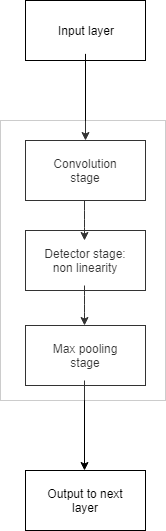
\includegraphics[width=4cm, height=10cm]{img/data/imagecnnlayer.png}
	\caption[]
	{Components of the convolutional layer. Generally in the first layer, several convolutions are performed in parallel to generate a set of linear activations.  Next each linear activation generated will be applied to a nonlinear activation function, in our case the rectified linear function called ReLU. In the pooling layer, a pooling function is used in order to manipulate the output of the layer.}
	\label{fig:imagecnnlayer}
\end{figure}\par

The layers of a convolutional neural network which are neither the input nor the output layer are called hidden layer. Practically these are the layer that do all the computation and whose operations was described above.  These hidden layers have the structure of the convolutional layer pictured in figure (3.1). The filtering stage was discussed, the pooling stage was discussed, but now the need for discussing the activation stage (non linearity stage) arises. This stage is also called "hidden unit" of the hidden layer. There are several choices for an activation function, but the more usual ones are softmax(Standard softmax function, $\sigma:\Rrr->\Rrr$, eq 3.10), tanh(eq 3.11) and rectified linear (ReLU eq 3.12), described in the equations below: 

\begin{equation}
    \sigma(x)=\frac{e^{x}}{\sum^{n} e^{x}}
\end{equation}

\begin{equation}
    tanh(x)=\frac{e^{2x}-1}{e^{2x}+1}
\end{equation}

\begin{equation}
    ReLU(x)=max(0,x)
\end{equation}

The design process of choosing which suits best your architecture is usually done by trial and error. In my case, choosing ReLU for the defect detection prototype was done by the virtue of emulating the VGGNet architecture \cite{article-vgg}. A single potential problem arises when using rectified linear. It is the fact that at the point x=0, the function is not differentiable. But, SGD performs good enough in order to use ReLU in CNN models. The fact that SGD still works in these conditions is given by the fact that the algorithm does not exactly arrive in the local minima, but gets to a place which is a mere approximation of the local minima.\par

In the convolutional neural network, most hidden layers are described by the following equation in which u is the input vector, x is the output, b is the bias and W are the weights of the connections:

\begin{equation}
    x=W^{t}u+b;
\end{equation}

The use of ReLU is depicted in the equation below. Y is the value for the neuron of the next layer:

\begin{equation}
    y(x)=ReLU(W^{t}u+b;)
\end{equation}

Only after this part of the computations has been done, the rectified linear activation is applied. Moreover, it is easy to optimize this activation function because it is similar to linear ones. This yields the fact that the derivatives through half the domain remain large whenever the unit is activated. Also, it is trivial to mention the fact that the second derivative is 0 in almost every single point. The single drawback on using ReLU activation is the fact that the networks cannot learn by using gradient based optimization algorithms on datasets for which their activation is 0. This is solved by the generalizations of rectified linear unit function but they are behind the scope of building the prototype and will not be discussed.\par

The last operation used is the dropout, which is not mandatory to occur at every layer of the CNN but it helps with introducing redundancy into the neural network model because not a single neuron in the layer is responsible for predicting a certain class. Thus providing an inexpensive way of regularizing a large variety of models. Dropout is usually performed at a rate of dropping out 40-50\% of the neuron in the fully-connected layers and at a much lower rate, 10-25\% in all the convolutional layers. It should be mentioned the fact that not all hidden layers are convolutional layers, there can also be fully-connected layers that are hidden layers. But if we have convolutional layers in the network model, they are hidden layers. The terminology could be confusing.\par

It shall be mentioned the fact that these modern network types can be very deep, more than 10-20 layers and by having this depth they can derive lots of features and abstractions, creating an inference engine that is capable of out-performing humans in certain vision-based tasks such as object detection

\subsection{R-CNN a better version of CNN}
A more modern approach of detecting object in images and performing image segmentation is the region based CNN\cite{article-rcnn}.
R-CNNs improve the mean average precision by more than 30\% when tested on the Pascal VOC dataset benchmark, achieving 53.3\%. This is well beyond what normal CNN based solution obtained on the same dataset. This is possible because they make use of two improvant properties:
\begin{itemize}
    \item They apply a high-capacity CNN to bottom-up region proposals in order to locate and segment objects
    \item They can get a significant improvement for accuracy when there is not sufficient labeled training data, thus they use a supervised pre training for an auxiliary task, followed by a domain specific fine tuning.
\end{itemize}

They work by taking the input image, and extracting from it 2000 bottom-up region proposals. Then, the algorithm computes the features for each region proposal using a large CNN. Finally, it classifies each region using a class specific linear support vector machine (SVM). Therefore it can be said that this algorithm consist of three modules, all encompassed into one solution.

\textbf{Remark:}In order to be able to use the full benefits of R-CNNs, one shall have appropriate hardware setup. Having in mind that this prototype was a proof-of-concept and that there exist hardware constraints I did not use R-CNN in developing the solution because it would slow down the actual progress. Also, it should be pointed out that this is a very quick way to improve the overall speed and accuracy if the hardware is appropriate.


\section{Data set and traning}
In order to make use of the full computational power of convolutional neural networks, one shall use a large and labeled dataset. I needed to create my own data set based on the very small data set received from the contractor: OKOS SOLUTION. They supplied around 30 digital images describing the defects that can appear on the component housing. The number of initial images was too small. They also told us how to augment the images/simulate the defects with a photo augmenting software on the respective new images that we will create. The process was simple and it consisted out of two steps:
\begin{enumerate}
    \item Copy all of the defect-free images several time, with modified brightness, contrast or slight rotations. Thus it results the positives. 
    \item Copy all of the defect-free images several time in the negatives folder. Then augment them in order for them to have similar pixels indicating defects as the negatives supplied by them have. The only catch is that they need to be in all the different position, but have the same or almost the same pixel structure.
\end{enumerate}

Finally, it resulted a total dataset count of 600 good images, 600 bad images, made with portability in mind (model should not be too big as it should be also implementable on micro-controllers). Moreover, in order for the data to be correctly labeled, it was split into two folder: good and bad. Labeling is important because when using supervised deep learning, it is important to specify which object appears in each of the digital input images. Both, labels and collection of features are important parameters of a good input dataset. Also, labeling can be done by numerical encoding, specifying 0=bad housing or 1=good housing, or by character encoding writing good or bad next to the analyzed image. It solely depends on the hardware capabilities of the machine on which the solution will be implemented. But, numerical encoding was not used in order to develop this prototype.

\subsection{Data set use}

Almost all deep learning algorithms experience a dataset, whether is it a fixed dataset or not (e.g. an environment). A common way of describing a dataset is with a design matrix, which is a matrix that contains different examples in each of its rows. Each of its columns corresponds to a specific feature. If m is the number of examples and n is the number of features, this design matrix (X) which mimics the dataset can be declared as $X \in \Rr$. It must be remarked that in order to apply this way of picturing the dataset, it must be possible to describe each example of the dataset as a vector and each vector must be the same size with the other. Well, this is not always possible, hence this solution is not a general one. In the mentioned case of defect detection, if the digital images fed as input, would vary in pixel size, this description would not be possible and other methods of handling such kind of heterogeneous data should be applied. But, in the mentioned case, all the fed images are of the same pixel size. In the figure \ref{fig:chartcapacityerror} one can see the relationship between the capacity of the dataset and the error of the dataset and the conditions of under-fit and over-fit. In the lefthand side of the chart as there are fewer training examples, one can see that the model underfits the test data while on the righthand side the model overfits the test data. The sweetspot is in the middle of the chart, where also the test error is minimized.

In order to move forward with the training procedure and to be able to further mathematically manipulate the algorithm (somehow correlating test and training errors), several assumptions need to be made. Firstly, the examples in the dataset are independent from each other. Additionally, the training dataset and the test dataset are identically distributed, collected from the same probability distribution. These two assumptions enables the description of the data-generating process in form of a probability distribution over a single set. An obvious connection that can be seen between the training errors and the test error is the fact that the expected value of the training error of a randomly selected model is equal to the expected value of the test error of that specific model.


\begin{figure}[h!]
	\centering
	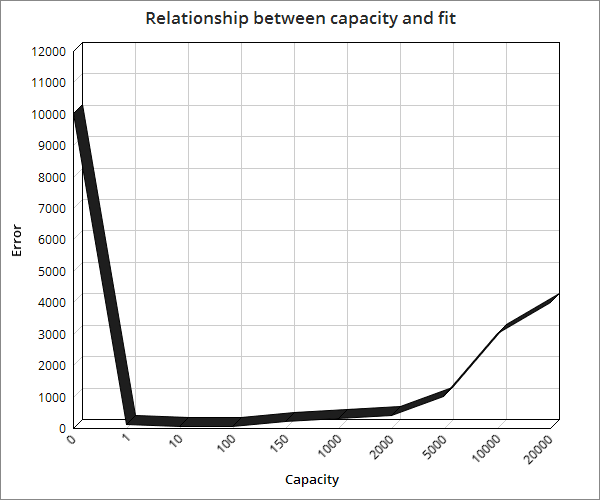
\includegraphics[width=12cm, height=6cm]{img/data/chartCapacityError.png}
	\caption[]
	{The relationship between capacity and generalization error. As one can see 100 is the optical capacity for which the smaller error is generated. This is not on the actual dataset, but is a general case.}
	\label{fig:chartcapacityerror}
\end{figure}


\subsubsection{Data types used in CNNs}
Data points in the dataset used in solutions trained with CNNs generally consist of several channels, every channel being the observation of a different feature at some point in space or time. The images used are 2D data points with multiple channels. The channel configuration is RGB: red, green, blue. To be mentioned the fact that the conv filter kernel slides over the 2D plane, assuring translation equivariance in both dimensions. In the manufacturing process mentioned we find the case where every training example and every test example has the same spatial dimensions. Even if CNNs can process inputs with different spatial dimensions, there is no need to use this property now, but it is very useful for further developments. By the spatial dimensions of an digital image we usually refer to as the width and height.



\subsection{Training procedure}

What differentiates a deep learning algorithm from an optimization problem is the fact that the generalization error (test error) should also be as small as possible, not only the training error, as in the case of optimization. The generalization error of a deep learning algorithm is measured on a test set of examples, collected separately from the training set or collected together but uncorrelated.\par

The factors mentioned in the above section that determine the "goodness" of machine learning algorithms are: making the training errors as small as possible and reducing the gap between the training and test error. These two factors correspond to the two characteristics of deep learning algorithms, that are viewed as constraining factors: over-fitting and under-fitting. Over-fitting is a phenomenon that occurs when the difference between the training and the test error becomes too large, while as under-fitting is stated when the training error fails to yield a sufficiently low value. A general rule of thumb in order to handle fitting problems is to never have more parameters than training examples, but also not too few. One can manipulate the model in such way that it is more likely to over-fit or under-fit by manipulating its ability to fit a wide array of functions, also known as capacity. By changing the capacity, one changes the set of functions that the machine learning algorithm can select as the specific solution for the problem, also known as the hypothesis space. This space is not only influenced by choice, but also by the fact that the model specifies which set of functions the machine learning method can choose when varying the parameters. This sort of on-line choosing is called the representational capacity of the model. Generally, the algorithm performs best when the capacity is correlated with the amount of training data available and the complexity of the problem that needs to be solved. All in all, the algorithm does not find the best function that fits the criteria, but it find a function or a set of functions good enough such that it greatly reduces the training error of the model. This drawback should be payed attention to, because it often results that the effective capacity of the algorithm is less than the representational capacity of the model`s set. Also, it shall be remembered the fact that training and testing error vary as the size of the training input set varies.\par
In order to be able to train the convolutional neural network there is a need to compute the gradient with respect to the filter kernel used, from the gradients with respects to the outputs that are known a-priori. In some of the most trivial cases, this calculation can be performed by the means of the convolution operation. Besides trivial cases, there are also more complex cases, when filter strides are greater than 1, for which this approach does not yield a good result. Therefore there is a need for a third operation that can solve this problem, usually back propagation. Generally, these two operations: convolution and back propagation (from input to outputs and from outputs to inputs) are enough to calculate all the gradients needed to train any kind of deep convolutional neural network, as well as other type of deep networks.\par
Moreover, in order to get from the inputs to the outputs in a CNN one does not only use linear operations. Generally there exists also a bias term that is added to each output before applying the nonlinear activation function. For conv layers it is usually accepted to have one bias per channel of the output and share it between all locations within the conv feature map. Therefore a quick recap of the back-propagation algorithm is needed:\par

\subsubsubsection{\textbf{Backpropagation}} is the main algorithm of how feed forward neural networks learn, but is is only a part of the whole learning process. It consist of computing the negative gradient of the cost function. This shows how the cost function reacts to different weights and biases, such that one can minimize most efficiently the cost function. The idea behind using it is the fact that in feed forward networks the input provides information and this information generates an initial output guess. With the help of all these initial output guesses the cost function`s value is computed. Backpropagation enables this information to flow from the cost function through the network in order to compute a better gradient, hence it results the name. For the first procedure mentioned, the name is forwardpropagation. The magnitude of each component of the cost function tells how sensitive this cost function is to each weight and bias. A larger value for a component means that the cost function is more sensitive to its change in value than it would have for a smaller value component. In order for this method to work, it needs a lot of labeled training data. In order to learn, the network combines backprop with stochastic gradient descent.
Backprop is mathematically pictured by using the Chain rule of calculus, which states that:
\begin{equation}
    \frac{dx}{dz}=\frac{dx}{dy}\frac{dy}{dz}
\end{equation}

Thus, backpropagation is obtained by applying the chain rule recursively:

\begin{algorithm}[h!]
\SetAlgoLined
\KwResult{Gradient table completed with the gradients }
 Run forward propagation to obtain the activations of the network;\\
 Initialize the table of gradients gradtable;\\
 gradtable[u^{n}]=1;\\
 j=n-1;\\
 \For{j>=1}{compute
 $\frac{\partial u^{n}}{\partial u^{j}} = \sum_{i} \frac{\partial u^{n}}{\partial u^{i}}\frac{\partial u^{i}}{\partial u^{j}} $ \\
 gradtable[u^{j}]=\sum_{i}gradtable[u^{i}] * \frac{\partial u^{i}}{\partial u^{j}} \\
 }
 \caption{Basic backpropagation implementation for computing the derivatives of $u^{n}$ with respect to the parameters. All variables are chosen scalars for simplicity. The computational cost of the algorithm is proportional to the number of edges in the graph that depicts the input structure. The algorithm is cited from \cite{book-deeplearning}.}
 
\end{algorithm}

Moreover, when starting the training process the parameters need to be initialized. Usually a random initialization would not get us far for the number of epochs parameter and the initial learning rate parameter. An epoch is an instance where the network, while training, sees the data and derived information from it, hence the total number of epoch is how many times the CNN analyzes each training example and learns patterns and features from it. There is no exact number of epoch for which a training procedure should last. It is done usually by trial and error, by noting different patterns from the graph that results after training and noticing the accuracy patterns. The initial learning rate is usually initialized at 1e-3, because is it the default value for the Adam optimization process. More will be discussed about the learning rate in the next sub-section.\par


\subsubsection{Stochastic Gradient Descent "SGD"}
A well known approach for optimizing deep learning training procedures is the stochastic gradient descent, which is an iterative method. It is an extension of the classical gradient descent optimization algorithm. Generally, for classical gradient descent the computational cost of the operation is O(n), where n is the total number of samples. Stochastic Gradient Descent proved to be a very efficient optimization algorithms that was started being used in many machine learning and deep learning applications, because it is suited for the computational overcharge that the large datasets that are being used generate. The term stochastic comes from the property that the objective function may be composed out of a sum of sub-functions evaluated at different sub-samples of data. The gradient becomes an estimation, on these mini-batches of examples drawn from the training set. Usually the size of the mini-batch is chosen to be small, thus enabling a good approximation of the gradient. It is important as to not increase the size of the mini-batch, even if the overall training set increases. If we consider that n` is the size of the mini-batch, C is the cost function, x are the examples and y is the output, $\theta$ are the parameters, we can write the following equation that describes the operation:

\begin{equation}
    g={(1/n`)\nabla_{\theta}\sum_{i=1}^{n`}C(x(i),y(i),\theta)}
\end{equation}
Furthermore, the SGD algorithm follows the downhill pattern of the computed gradient, where $\epsilon$ is the learning rate chosen:
\begin{equation}
     \theta = \theta - \epsilon*g
\end{equation}

The learning rate is the speed by which the value of the gradient is modified (shrunk). There exist a lot of work in the approaches of optimizing the use of the method of gradient descent in deep learning. Other implementations of GD have been documented such as:
\begin{itemize}
    \item AdaGrad 
    \item RMSProp
    \item Adam
    \item Natural Gradient Descent
\end{itemize}


\subsubsection{Adam optimizer}
Adam optimizer\cite{article-adam} is a first order gradient based optimization of stochastic objective function based on adaptive estimates of lower order moments. It is modern and vastly used in the engineering field because it is straight forward to implement and it very efficient computational wise. Moreover, by having the following enumerated properties it is extremely well suited for problems that have a lot of parameters and a lot of data, hence it is well suited for image recognition problems. Its advantages are:
\begin{itemize}
    \item it works well with sparse gradients
    \item it works well in an online and non stationary setting
    \item it is invariant to the re-scaling of the gradients
    \item it has bounded step-sizes dictated by the step-size hyperparameter, which also requires very few tuning
    \item it doesn`t require a stationary objective
    \item it performs a form of step-size annealing
\end{itemize}
\textbf{Remark:} I will not treat the convergence proof of the algorithm. You can find it in the cited article above.\par
Below, the algorithm is outlined. The only conditions are that f be an objective function that is differentiable with respect to its parameters $\theta$. The result should be the parameters for which the function is minimized at time step t. The stochasticity comes from the computation at random time instances of minibatches of datapoints or from the inherent function noise. There should be mentioned the fact that $\nabla$ represents the gradient:

\begin{algorithm}[H]
\SetAlgoLined
\KwResult{Returns the resulting parameters $\theta$ at time step t}
 initialization of $\alpha$;  $\beta_{1}$; $\beta_{2}$; $\theta$; \\
 initialization of parameter vector, moment vectors and time step t; \\
 \While{$\theta(t)$ not converged}{
  t=t+1;\\
  g_{t}=\nabla_{\theta} f_{t} (\theta)_{t-1};\\
  m_{t}=\beta_{1} m_{t-1} + (1-\beta_{1}) g_{t};\\
  v_{t}=\beta_{2} v_{t-1} +(1-\beta_{2}) g_{t}^2;\\
  \^{m}_{t}=m_{t}/(1-\beta^t_{1});\\
  \^{v}_{t}=v_{t}/(1-\beta^t_{2});\\
  \theta_{t}=\theta_{t-1}-\alpha * \hat{m}_{t} / (\sqrt{ \hat{v}_{t}} +\epsilon);\\
  \textbf{return} $\theta(t)$;
 }
 \caption{Adam optimization. $\alpha$ is the step size parameter. $\beta_{1}$, $\beta_{2}$ are exponential decay rates for the moment estimates. f($\theta$) is the stochastic objective function with the parameters $\theta$ }
\end{algorithm}



\chapter{Design and implementation}
\label{ch:design}
\section{System overview}
The prototype was designed in order to comply with the constraints specified in chapter 1, section 1.3. The design process was split into three sub systems:
\begin{itemize}
    \item Implementing the CNN such that it complies with the constraints
    \item Training and testing
    \item User interface
\end{itemize}

A class diagram that overviews the system and shows the inherent relationships is presented in figure 4.1.


\begin{figure}[h]
	\centering
	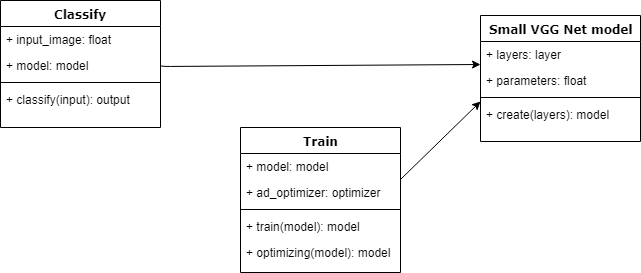
\includegraphics[width=13cm, height=5cm]{img/data/imagesystem.png}
	\caption[]
	{The general overview of the implemented system in Python.}
	\label{fig:imagesystem}
\end{figure}\par


\subsubsection{Data set augmentation}
In order to be able to use the supervised learning methods described in the theoretical background chapter, there is the need for a well labeled dataset. In order to comply with the specifications of the contractor, we will split the data into two folders, each folder with its own label: good and bad. Being the fact that I only received around 30 digital images and the final data set that I created has around 600 bad image examples and 600 good image examples, I will apply augmentation procedures on these images such that the training data will have higher variance. The following sequence of code depicts the function "ImageDataGenerator" from the Keras library used in order to augment the input images. It generates batches of tensor image data with real-time data augmentation. It will be looped over in batches.

\begin{lstlisting}[language=Python, basicstyle=\small, caption={Data augmenting script},captionpos=b, label=code:datapreparation]

import keras
#data augmentation
aug = ImageDataGenerator(rotation_range=25,
width_shift_range=0.1,	height_shift_range=0.1,
shear_range=0.2, zoom_range=0.2, horizontal_flip=True, fill_mode="nearest")
\end{lstlisting}

The parameters of the function have the following meaning:
\begin{itemize}
    \item rotation range - inputs the degrees range for random rotations
    \item width shift range
    \item height shift range
    \item shear range - inputs the Shear angle in counter-clockwise direction in degrees for shear intensity
    \item zoom range - the range for random zoom
    \item horizontal flip - if true it randomly flip inputs horizontally
    \item fill mode - Should be put one of the following {"constant", "nearest", "reflect" or "wrap"}. Default is 'nearest'. Points outside the boundaries of the input are filled according to the chosen mode.
\end{itemize}

When training the network the method "flow" will be called of the ImageDataGenerator class will be called which takes the input data and label arrays and generates batches of augmented data of a chosen size. The size chosen will be 32, but it is determined by trial and error and depends on the application. It is possible that the algorithm runs as well with other value of the batch size parameter.\par
The folder structure is briefly presented in the figure \ref{fig:imagesystem1} below:

\begin{figure}[h]
	\centering
	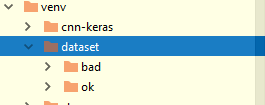
\includegraphics[width=7cm, height=4cm]{img/data/databasestructure.png}
	\caption[]
	{The general overview of the database structure.}
	\label{fig:imagesystem1}
\end{figure}\par

And the structure of the sub-folder of negatives is picture in figure\ref{fig:folders}. The positives one is analogous:\par

\begin{figure}[h]
	\centering
	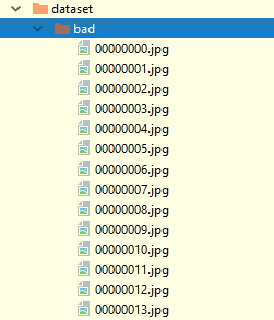
\includegraphics[width=10cm, height=8cm]{img/data/databasestructure1.png}
	\caption[]
	{The general overview of the sub-folders.}
	\label{fig:folders}
\end{figure}\par

Moreover the image that we need to detect is pictured below. One example is a clean image without defect \ref{fig:exemplu1} and the other is an image that presents defects\ref{fig:exemplu2}. The defect shall be explained a little bit here. A defect is considered when there exists a larger than 3-4 pixels area of a shade of grey on the exterior wall of the housing. This structural defect is only visible by acoustic microscopy and it generates leaks, thus it compromises the structural integrity of the housing and it need to be picked up at quality checking before generating more harm:

\begin{figure}[h!]
	\centering
	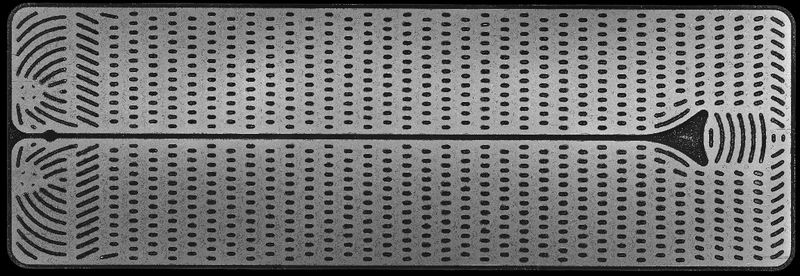
\includegraphics[width=13cm, height=5.5cm]{img/data/good_ex1.jpg}
	\caption[]
	{An example of a defect free housing image. This should be a good piece and should continue down the manufacturing pipeline.}
	\label{fig:exemplu1}
\end{figure}\par


\begin{figure}[h!]
	\centering
	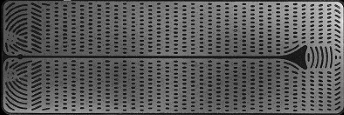
\includegraphics[width=13cm, height=5.5cm]{img/data/exemplu_imagine2.jpg}
	\caption[]
	{This image is an example of a defect housing image. This should be a bad piece and should not continue down the manufacturing pipeline. One can clearly see the defect on the upper left hand side of the plane with a shade of grey. This is considered a defect and needs to be picked up.}
	\label{fig:exemplu2}
\end{figure}\par


\section{Network implementation \& implementation modules}
In this section the network architecture chosen will be described: how it will be implemented, which are the modifications made such that it obeys to the initial specifications ordered by the contractor and what is the idea behind using this type of architecture. Moreover, I will briefly pass through each implementation module used for implementing the CNN in the Python programming language on the Windows 10 operating system, with the Keras library. These are the needed imports for all implementing the neural network model:

\begin{lstlisting}[h!][language=Python, basicstyle=\small, caption={Importing the necessary libraries. Keras documentation is the most important and can be found \href{https://keras.io/}{\textbf{here} },captionpos=b, label=code:datapreparation]
from keras.models import Sequential
from keras.layers.normalization import BatchNormalization
from keras.layers.convolutional import Conv2D
from keras.layers.convolutional import MaxPooling2D
from keras.layers.core import Activation
from keras.layers.core import Flatten
from keras.layers.core import Dropout
from keras.layers.core import Dense
from keras import backend as K
 
\end{lstlisting}



\subsubsection{Neural network model implementation}
Because the problem is a image classification problem at heart (even if it is called defect detection, the basics are that of a classifying algorithm, classifying the images into defect and defect-less images), I chose to implement a variation of the very deep CNN architecture called VGGNet developed by Karen Simonyan \& Andrew Zisserman\cite{article-vgg}.
VGGNet is a CNN architecture that makes use of small 3x3 conv filters instead of larger ones and increases the depth of the network up to 16-19 layers. Analyzing the presented results in the paper one can see that it obtains good performances and good enough generalization. Moreover, the input of the network is a fixed size image, which is then passed through a stack of convolutional layers where the small receptive field are used. The filter size was chosen as mentioned, because it is the smallest dimensional filter that percepts the notions of left, right, up, down and center, while the stride size used for the filter is 1. They all have a relatively small width, starting with 32, then increasing up to 128. Furthermore, the spatial pooling is carried out by three max pooling layers. The size of the pool kernel is 3x3 and 2x2, reduced after the first use in order to not reduce the spatial dimensions too quickly. The spatial padding of the conv layer input is done in such way that it maintains the spatial resolutions after convolution. I also used 2 fully connected layers for classification. Even though in the original architecture they propose making use of 3 such layers, I needed to reduce the number of layers in order to satisfy the hardware constrains. The first one has 1024 channels, while the second one has one or two channels depending of the loss function used: sparse categorical cross entropy - 1 channel or for binary crossentropy - 2 channels. Finally, the last layer is a softmax classifier. All hidden layers implemented use the ReLU activation function. No local response normalization was used because normalization does not improve the performances in such a way that it is worth it. But what is does it increases the memory needed, hence it increases the computation time. So it is not a trade off worth making.

\begin{lstlisting}[h!][language=Python, basicstyle=\small, caption={Code sequence for implementing a CNN layer. The first line of code is the function called for implementing a conv layer. The second one is the implementation of the activation function ReLU. Then max pooling is implemented and finally dropout. The parameters configurations can be easily found in the online documentation of the keras library, \href{https://keras.io/}{\textbf{here} },captionpos=b, label=code:datapreparation]

model.add(Conv2D(32, (3, 3), padding="same",
		input_shape=inputShape))
model.add(Activation("relu"))
model.add(BatchNormalization(axis=chanDim))
model.add(MaxPooling2D(pool_size=(3, 3)))
model.add(Dropout(0.25))
 
\end{lstlisting}

\begin{lstlisting}[h!][language=Python, basicstyle=\small, caption={Code sequence for implementing the final FC classification layer. The Dense parameter can be 1 or 2 depending on the chosen loss function. The parameters configurations can be easily found in the online documentation of the keras library, \href{https://keras.io/}{\textbf{here} },captionpos=b, label=code:datapreparation]

model.add(Flatten())
		model.add(Dense(1024))
		model.add(Activation("relu"))
		model.add(BatchNormalization())
		model.add(Dropout(0.5))
 
		model.add(Dense(1))
		model.add(Activation("softmax"))
 

		return mode
 
\end{lstlisting}



\subsubsection{Specifics for VGGNet}
Comparing this architecture with other architecture in the literature one can see that others are using larger convolutional filter kernels. By having for example a 7 × 7 effective filter kernel the network can pick up better defined features. But a 7x7 kernel can be also made out of a stack of three 3x3 convolutional layers. Also, in the latter case we use three non-linear ReLU activation layers instead of a single one, which improves the decision making by enhancing the discriminativeness of the decision function. Additionally the number of parameters are decreased: assuming that both the input and the output of a
three-layer 3 by 3 convolution stack has C channels, the layer has $27C^{2}$ weights, while the approach with a 7 by 7 conv. layer would require $49C^{2}$ parameter, more than 80\% more parameters. This also increases the computation time. Hence using more and smaller conv filters is an important advantage.



 
    
\section{Training and testing}
The training procedure was described in the Theoretical background chapter. By using the keras library one can easily implement the procedures mentioned:

\begin{lstlisting}[h!][language=Python, basicstyle=\small, caption={Necessary imports in order to train the network. All libraries are open-source ones.},captionpos=b, label=code:datapreparation]

 
from keras.preprocessing.image import ImageDataGenerator
from keras.optimizers import Adam
from keras.preprocessing.image import img_to_array
from sklearn.preprocessing import LabelBinarizer
from sklearn.model_selection import train_test_split
from pyimagesearch.smallervggnet import SmallerVGGNet
import matplotlib.pyplot as plt
from imutils import paths
import numpy as np
import argparse
import random
import pickle
import cv2
import os
import matplotlib
matplotlib.use("Agg")
\end{lstlisting}





\begin{lstlisting}[h!][language=Python, basicstyle=\small, caption={Training procedure code sequence. The parameter configurations can be found online in the keras documentation. Remark: the loss function is binary crossentropy or sparse categorical crosssentropy depending on the desired method. Both were tested, only one is used.},captionpos=b, label=code:datapreparation]



model = SmallerVGGNet.build(width=IMAGE_DIMS[1], height=IMAGE_DIMS[0], depth=IMAGE_DIMS[2], classes=len(lb.classes_))
opt = Adam(lr=INIT_LR, decay=INIT_LR / EPOCHS)
model.compile(loss="sparse_categorical_crossentropy", optimizer=opt, metrics=["accuracy"])

H = model.fit_generator(
	aug.flow(trainX, trainY, batch_size=BS),
	validation_data=(testX, testY),
	steps_per_epoch=len(trainX) // BS,
	epochs=EPOCHS, verbose=1)
 
\end{lstlisting}

The testing module is implemented in the model.fit generator. By plotting the inherent graph of the operation one can see the loss function and accuracy values.

    
\section{Classifying module}
As specified in the general overview, there is a need for a classifying module. This classifying module is easy to implement and is described in the code sequence below:

\begin{lstlisting}[h!][language=Python, basicstyle=\small, caption={Classifying procedure code sequence. The parameter configurations can be found online in the keras documentation.},captionpos=b, label=code:datapreparation]

from keras.preprocessing.image import img_to_array
from keras.models import load_model
import numpy as np
import argparse
import imutils
import pickle
import cv2
import os


image = cv2.imread(args["image"])
image = image.astype("float") / 255.0
image = img_to_array(image)
image = np.expand_dims(image, axis=0)

model = load_model(args["model"])
lb = pickle.loads(open(args["labelbin"], "rb").read())

classify_output = model.predict(image)[0]
idx = np.argmax(proba)
label = lb.classes_[idx]rbose=1)
 
\end{lstlisting}




\section{User interface}
For this project there was not dedicated user interface developed. But the Pycharm Professional IDE does a pretty good job, in a way that is it straight forward and has easy to use command. In the figure \ref{fig:imagesystemui}below the whole IDE is depicted with the more important commands highlighted: run, run setting and selecting the program. A dedicated user interface developed in Java will be included in the further developments section.
\begin{figure}[h!]
	\centering
	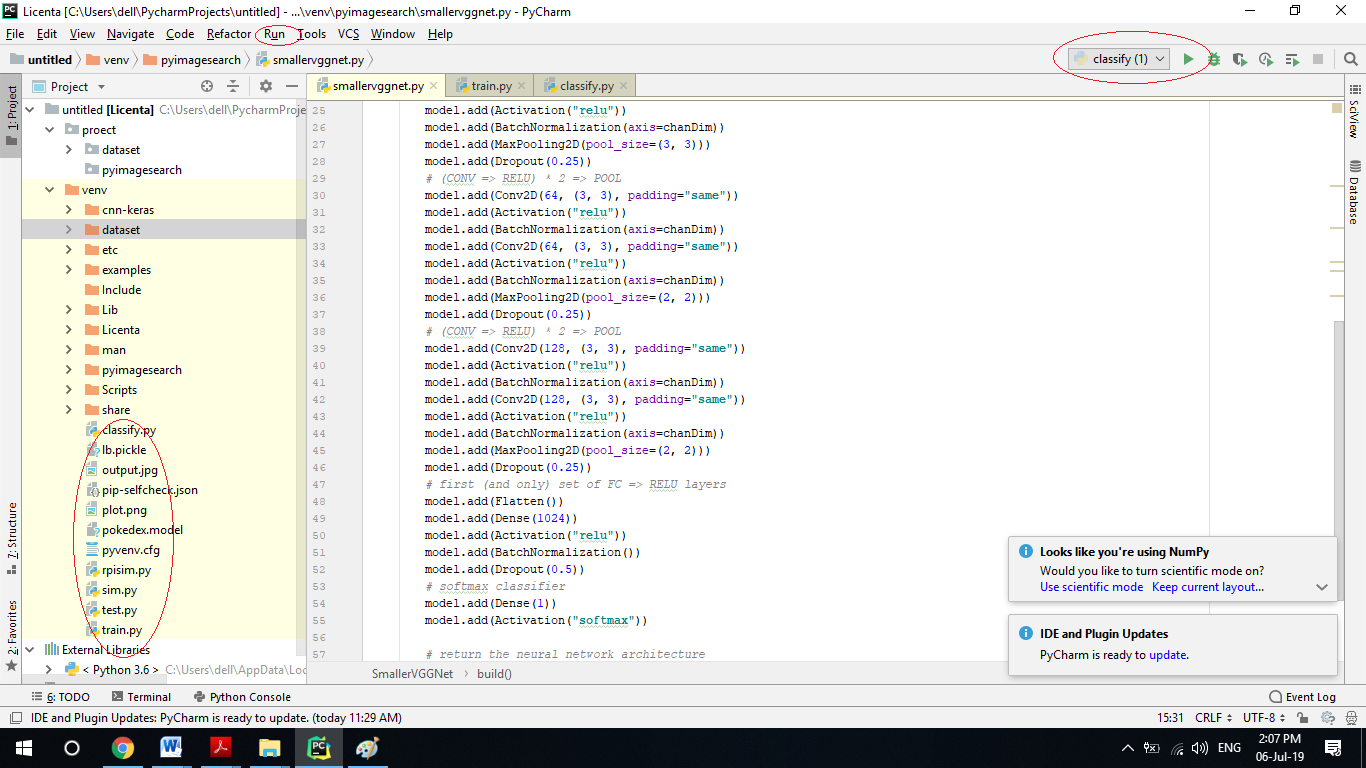
\includegraphics[width=12cm, height=7cm]{img/data/userinterface.png}
	\caption[]
	{The general overview of the Pycharm IDE.}
	\label{fig:imagesystemui}
\end{figure}\par


\chapter{Testing and validation}
\label{ch:results}
The validation of the neural network model will be made by taking into consideration the following performance aspects:
\begin{itemize}
     \item \textbf{Accuracy}, the number of times the network generally predicted the correct output
     \item \textbf{Classification time}, how much time does it take for the network to predict the output for one sample, not taking into consideration correctness
     \item \textbf{Training time}, how much time does it take for the network model to learn all the necessary features. Even though it is not a specification from the contractor, it still would be helpful to have information about it. 
\end{itemize}


\section{Testing}
The data was split in a 80/20 manner, meaning that 20\% of the data was used for testing and 80\% of the data was used for training. Moreover, in order to ensure a more robust model and a more "real" result, I also tested manually the model with another 100 images. The automatic testing was done by the already implemented function of the Keras library that also trains the model, specified in chapter 4, section 4.2. The result were read from a graph that was output from the procedure. The manual testing was done by hand, feeding each image to the network, one at a time. To be mentioned that the images are uncorrelated. Each sets of images is not related to the other, such that there is a natural variance in the data. In the following table \ref{tab:training_test} the data situation is depicted and a more optimal situation is presented in which more data is available. This kind of situation enhances the accuracy of the model, is a further improvement for the prototype, thus it is worth mentioning.

\begin {table}[h!]
\label{tab:training_test}
\begin{center}
 \begin{tabular}{|c |c| c | c|} 
 \hline
  & Nr. of training samples &  Nr. of test samples. & Total number\\ 
 \hline
 CNN model & 960 & 240 & 1200\\ 
 \hline
 CNN model target & 40,000 & 10,000 & 50,000 \\
 \hline
 \end{tabular}
\end{center}
\caption{Train-test split}
\end{table}

The following figures show how the manual testing was done, because the automatic testing was done in the same function call as the training and was mentioned in the chapter above it will not be mentioned here again. The sole idea of using the "argparse" library, which is a argument parser library as the name suggests, is the fact that we can run the program from the command window or from the Pycharm IDE \ref{fig:run1} and we can manually specify which image to feed into the program \ref{fig:run2}. This is very useful also in seeing how the network behaves, for debugging or in order to catch singularities of the software. First of all, one shall access the run settings from the navigation bar:

\begin{figure}[h!]
	\centering
	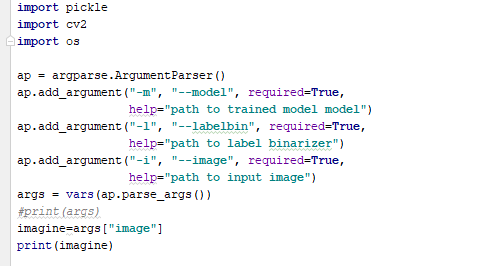
\includegraphics[width=12cm, height=7cm]{img/data/imagerun1.png}
	\caption[]
	{Overview of the Pycharm IDE navigation bar.}
	\label{fig:run1}
\end{figure}
\begin{figure}[h]
	\centering
	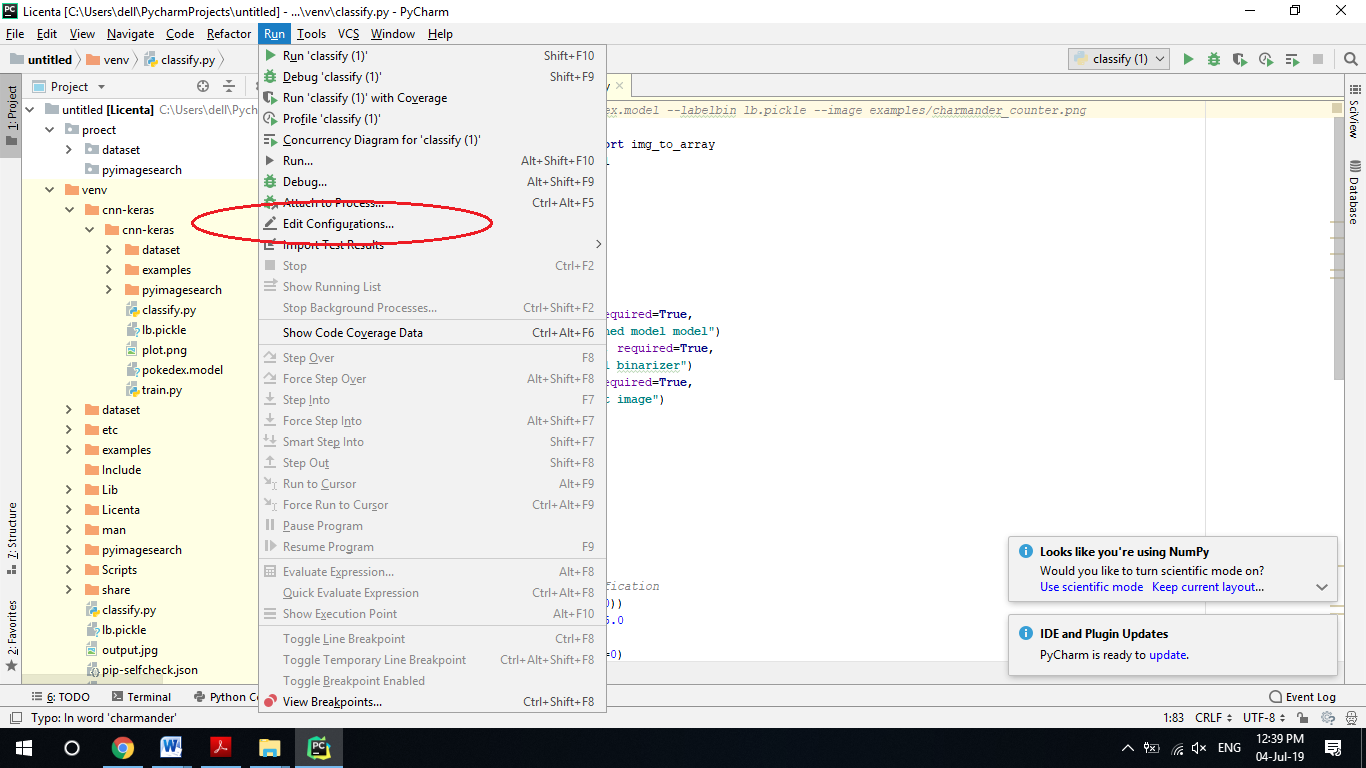
\includegraphics[width=12cm, height=7cm]{img/data/imagerun2.png}
	\caption[]
	{Overview of the Pycharm IDE.}
	\label{fig:run2}
\end{figure}

Special attention should be paid to the highlighted windows and forms. The name of the executed program should be verified and it should be verified that the script path is correct because otherwise errors could appear and they are hard to debug. Also, the correct arguments shall be introduced in the correct order. Otherwise the script will return an error. These fact are depicted in the figure \ref{fig:run3} below.
\begin{figure}[h!]
	\centering
	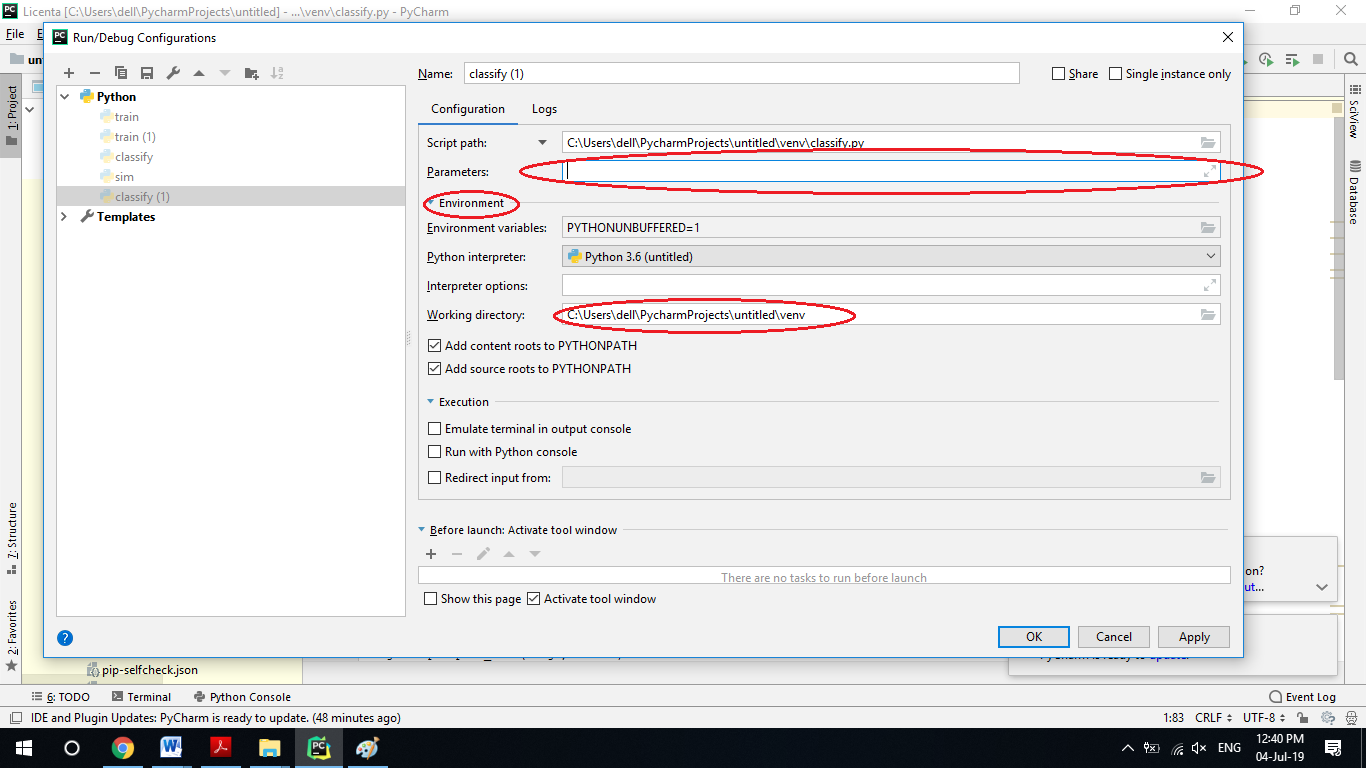
\includegraphics[width=12cm, height=7cm]{img/data/imagerun3.png}
	\caption[]
	{The general overview of the Run settings.}
	\label{fig:run3}
\end{figure}

\section{Analysis of the results} 
The results achieved should be analyzed in order to see which modifications yield a better model in the future and to be able to find the drawbacks of the actual one. In the figure \ref{fig:imaginerea} is pictured the result of feeding a defect housing image to the network. As we can see the network picked up the defect and returned to the user that the housing is defect, thus it did not pass the quality check test. In the figure \ref{fig:imaginebuna} we can see the result of feeding a defect free housing image to the network. As we can see the network classified this image correctly and thus it passed the quality check test.

\begin{figure}[h!]
	\centering
	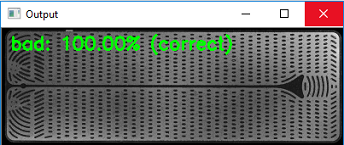
\includegraphics[width=12cm, height=6cm]{img/data/exemplu_imagine_gata.jpg}
	\caption[]
	{Result of a defect housing image with a sparse categorical cross entropy loss function and a single class. As one can see in the upper left hand side of the plane of the image there is a quite large area of a shade of grey. That is a defect and the network model picked it up.}
	\label{fig:imaginerea}
\end{figure}

\begin{figure}[h!]
	\centering
	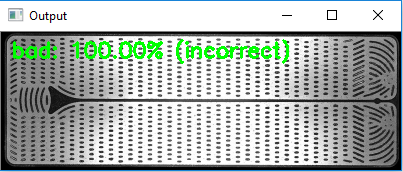
\includegraphics[width=12cm, height=6cm]{img/data/exemplu_imagine_gata_bun.png}
	\caption[]
	{Result of a defect free housing image with a sparse categorical cross entropy loss function and a single class in the output layer. The contrast is a little bit different as with the defect housing image, but as one can see there is no defect on neither sides of the image.}
	\label{fig:imaginebuna}
\end{figure}

Moreover, after training the network I plotted a graph with the received information from the training procedure in order to close a feedback loop with what the network was doing. This graph can be seen in figure \ref{fig:imaginegraf}.
\begin{figure}[h!]
	\centering
	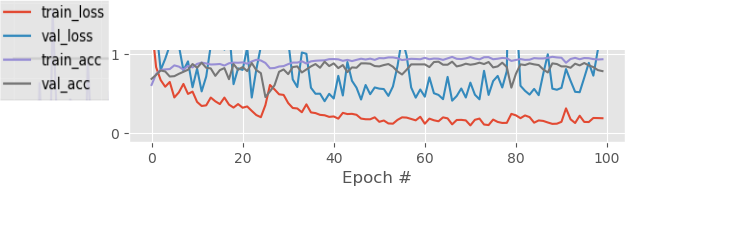
\includegraphics[width=15cm, height=6cm]{img/data/grafus.png}
	\caption[]
	{Result of training procedure with binary cross entropy loss functions. Here we can see the validation and the training accuracy. Validation accuracy = test accuracy. As we can see the test accuracy hovers around 77-80\% and it doesn't actually grow that much after the first 40 epochs, which shows us a bit of redundancy in the training process, as well as unnecessary computation.}
	\label{fig:grafus}
\end{figure}

\textbf{Remark:} Besides the fact that after the \nth{40} epoch, the test accuracy does not actually improve considerably, this is an example of a slightly under-fitting of the data generated by the fact that the dataset available was scarce and with bad variance. Also, this can be improved by a more deeper CNN model, as the image is large and it will pick up more definitive features.



\subsection{Conclusions}
The testing and validation was performed with the final goal in mind of validating the best obtained model as well as, finding patterns and further improvements that would yield a better model. Also, portability and integrability was taken into consideration obeying to the specifications of the contractor. 
The best obtained model is not just the model with the highest accuracy, but the model with the best overall performances of accuracy, classification time and training time (with a much smaller weight).
Performance metrics are found in the table below. \textbf{Remark}: by obtaining a better performing model we also increase its size, thus making it less portable and less adaptable to other applications. \textbf{Remark2}: Training time is affected both by architecture (depth-ness), as well as hardware setup. In my case, the hardware available is a bottleneck:


\begin {table}[H]
\label{tab:performance}
\begin{center}
 \begin{tabular}{|c |c| c | c| c|} 
 \hline
  & Accuracy &  Training time (h) & Classification time (sec) & Total images\\ 
 \hline
 CNN model & 77\%* & 960 & 10 & 1200\\ 
 \hline
 CNN model target & 95\% & 72-120 & <1 &50,000 \\
 \hline
 \end{tabular}
\end{center}
\caption{Performance metrics obtained. *the accuracy given is the mean accuracy because the manual testing data`s accuracy is 79-81\% while automatic testing`s accuracy is 75-77\%\%.}
\end{table}


\section{Validation}
Depending on the applications, there are different measures of performance, thus methods of validating the models, ensuring that the models are complying with the performance requirements.
Mentioning the validation methods. For classification we have accuracy and error rate.
Accuracy - the proportion of examples for which the model produces the correct output
Error rate - the proportion of examples for which the model produces incorrect output. Also refer to error rate as the expected 0-1 loss. It means 0 when it is correctly classified and 1 is it is not. \cite{book-deeplearning}
Generally, we are interested in how the deep learning algorithm performs on data that it has not seen before/ was not included in the training set, because this fact determines how well the algorithm will behave once it is deployed in the real world. Therefore, a need for a test and validation set, uncorrelated with the training set, arises. Furthermore in figure \ref{fig:imaginerea} one can see the result of feeding an image that represents a component housing with defects into the network algorithm. In figure \ref{fig:imaginebuna} one can see the result of feeding an image that depicts a housing without defects into the CNN. In figure \ref{fig:grafus} one can see the resulting graph from the training procedure that reproduces exactly every single loss and their evolution. This is very helpful in determining if the number of epoch are optimal and to see the evolution of the loss functions during training. This aspects were mentioned also in the section above, but should be mentioned again due to the displacement of images in the work.

Also there arises a big questions regarding real world accuracy? How should the model be penalized for making mistakes? Should be penalize each mistakes the same? Or should we penalize larger mistakes more than smaller mistakes? E.g. if the defect detection system says a good piece is faulty, should we be more forgiving in penalizing the model then when it says that a faulty piece is good? Judging by the fact that a false positive does more harm than a false negative, the best approach would be to penalize harder for false positive and to be more forgiving with false negatives.



\chapter{User guide}
\label{ch:guide}
In order to be able to use this CNN-based solution a minimal amount of guiding is needed. Moreover, to replicate the results and the training and testing steps mentioned above, at least the following hardware and software resources are needed:

\textbf{Hardware}
\begin{enumerate}
    \item a NVIDIA GPU with Compute Capability (CC) >= 3.0 
    \item a CPU with a working frequency >= 2.0 GHz and at least 8GB of RAM
    \item a stable and working internet connection
\end{enumerate}

\textbf{Software}
\begin{itemize}
    \item First of all, the user needs a version of Python 3.5 or higher
    \item Secondly, the user needs to decide which IDE he will use. The solution is compatible with the terminal version of Python3 and with the PyCharm IDE. One can download the PyCharm IDE from the internet.
    \item From the internet, CUDA and CUDNN compatible versions with the GPU the users has, need to be installed. I recommend CUDA Toolkit 9.0+ and CUDNN version 7.0+
    \item Once PyCharm is installed, one can easily download and install the following open-source Python libraries, depicted in figure 6.1:
    \begin{itemize}
        \item Tensorflow-gpu, here increased attention should be payed, because we want the tensorflow for gpus, not the tensorflow for cpus
        \item Keras 
        \item NumPy
        \item Matplotlib
        \item OpenCV
        \item Imutils
    \end{itemize}
\end{itemize}

In order to correctly install the CUDA Toolkit and the cuDNN library, one shall carefully read the instruction from the NVIDIA developer page, because the installing process is also important in order to be able to work with them! \par

\begin{figure}[h!]
	\centering
	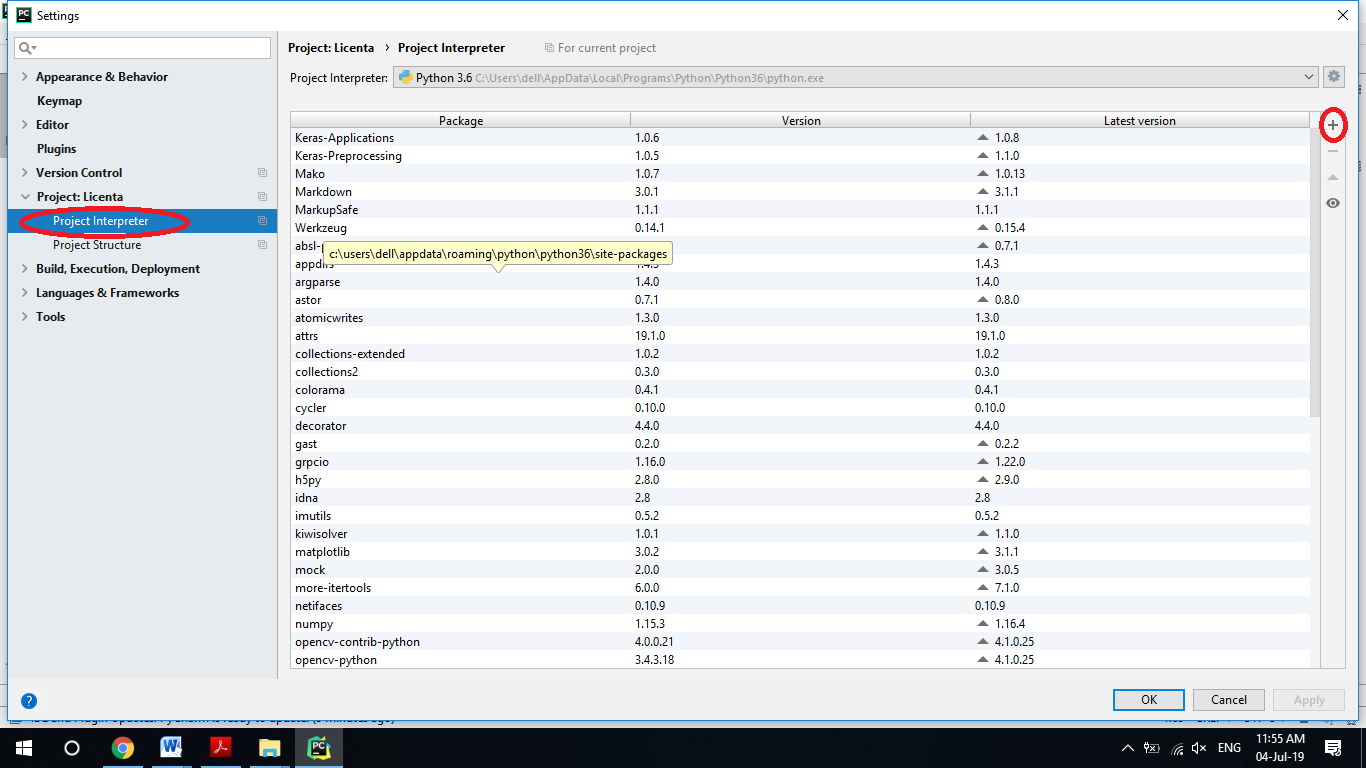
\includegraphics[width=15cm, height=9cm]{img/data/imagelibraryinstall.png}
	\caption[]
	{The window which opens when the user wants to install new libraries. Select File->Settings.}
	\label{fig:imagelibraryinstall}
\end{figure}


\section{Installation}
Steps for installation of Pycharm, all the libraries CUDA and cuDNN and other on Windows 10 OS. I recommend that firstly, one should be sure that the operating system has Python version 3.5+ installed and is compatible with the system. It your system does not have a Python version, you can install it from the website:  \href{https://www.python.org/downloads/}{downloadpython}. The install path and folders will be automatically set, once downloading. Also, one should download Pycharm from their \href{https://www.jetbrains.com/pycharm/download/}{website}.\newline

\textbf{Cuda \& cuDNN}\newline

The installing steps and guidelines can be found on the NVIDIA developers page \href{https://docs.nvidia.com/cuda/cuda-installation-guide-microsoft-windows/}{here}. Incrementally this version is updated each year or multiple times each year, so I recommend installing version 9.0. In order to be sure that the Toolkit was correctly installed, the user should have the following command line:\newline

\textbf{C:\textbackslash Program Files\textbackslash NVIDIA Computing Toolkit\textbackslash CUDA\textbackslash v9.0} \newline

\textbf{Remark}: If this path is not automatically set by your operating system it should be added to the environmental variables "PATH" of your Windows 10 operating system.

The cuDNN library (version 7.0), in zip format, can be downloaded from \href{https://developer.nvidia.com/cudnn}{here}. In order to be able to freely download it, the user need to create a NVIDIA account. It is free of charge and it takes around 2 minutes. Next, in order to install cuDNN the following steps must be respected:
\begin{enumerate}
    \item Unzip it into the folder "CUDA".
    \item In this CUDA folder, the user will find the sub-folders: bin, include and lib.
    \item The folder from the zip file with the names: "bin", "include" and "lib" will be copied into the pathway above mentioned. This concludes the installation process for CUDA and cuDNN.
\end{enumerate}

\textbf{Remark:} The libraries will all be installed through the Pycharm IDE because it is more user friendly and straightforward. However, if for some reason the user cannot find or install the needed packages the following alternative exists:\newline
\begin{itemize}
    \item Open windows command line
    \item Type "python get-pip.py"
    \item Type "pip install --upgrade tensorflow-gpu" 
    \item Type "pip install keras"
    \item Type "pip install matplotlib"
    \item Type "pip install numpy"
    \item Type "pip install opencv-python"
\end{itemize}

\section{Use}

Together with the documentation a CD was supplied with contains the relevant code. The user should open the PyCharm IDE and then link the folders contained in the CD with the working environment. After it there are 2 approaches:
\begin{enumerate}
    \item Run the program from the windows command line, which will be the final form of running this application when implemented in the manufacturing process on a micro-controller or compute on the edge stick. This involves opening the command line and then introducing the required parameters in order to enable the program to work. The required parameters are specified in the beginning of the program and are depicted in figure 6.2.
    \item Run the program from inside the PyCharm IDE. This method is very good for debugging and also it more computationally costly to use. It makes sense using it like this while converging to the final solution. The steps needed to perform this are depicted in the figures 6.3, 6.4 and 6.5.
\end{enumerate}

\begin{figure}[h!]
	\centering
	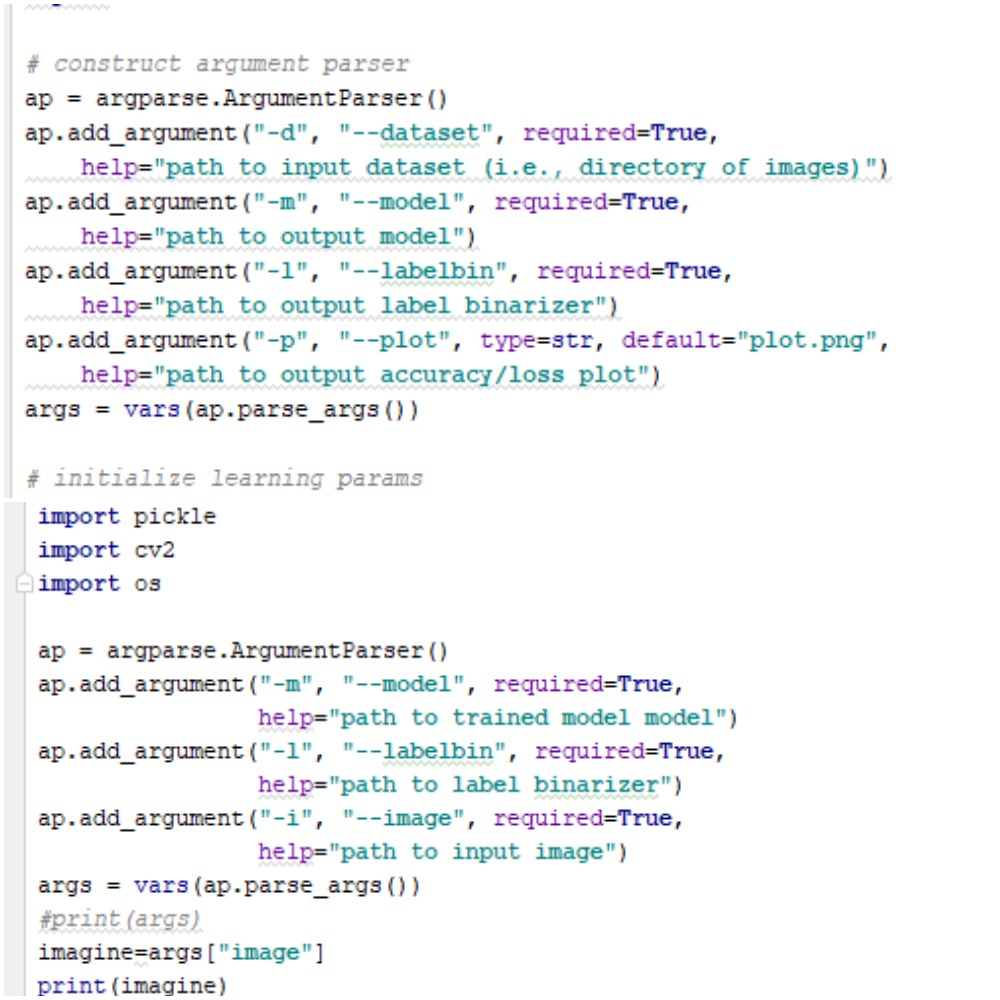
\includegraphics[width=15cm, height=10cm]{img/data/imagerun1.jpg}
	\caption[]
	{Required parameters in order to correctly run the programs. Both classification and training.}
	\label{fig:imagerun1}
\end{figure}

\begin{figure}[h!]
	\centering
	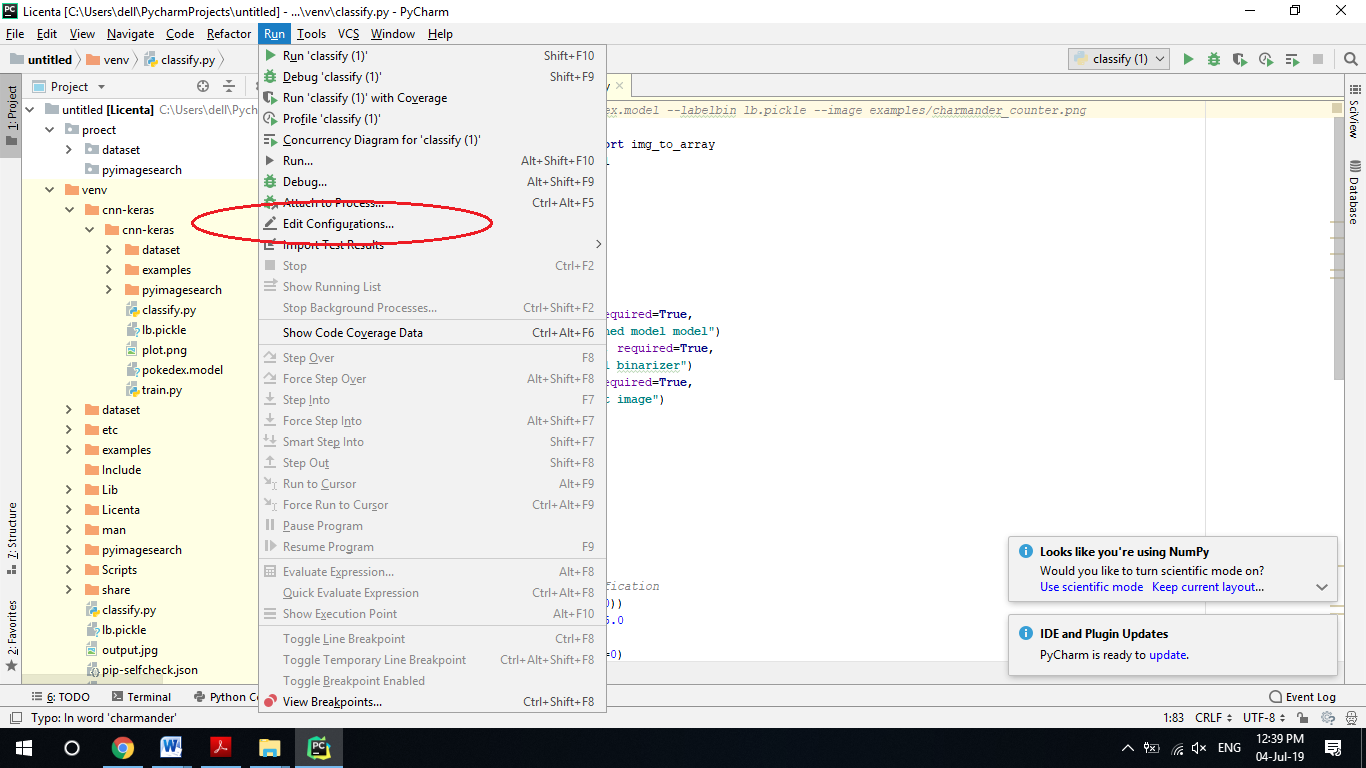
\includegraphics[width=15cm, height=9cm]{img/data/imagerun2.png}
	\caption[]
	{Open the Pycharm IDE and select Edit configurations.}
	\label{fig:imagerun2}
\end{figure}

\begin{figure}[h!]
	\centering
	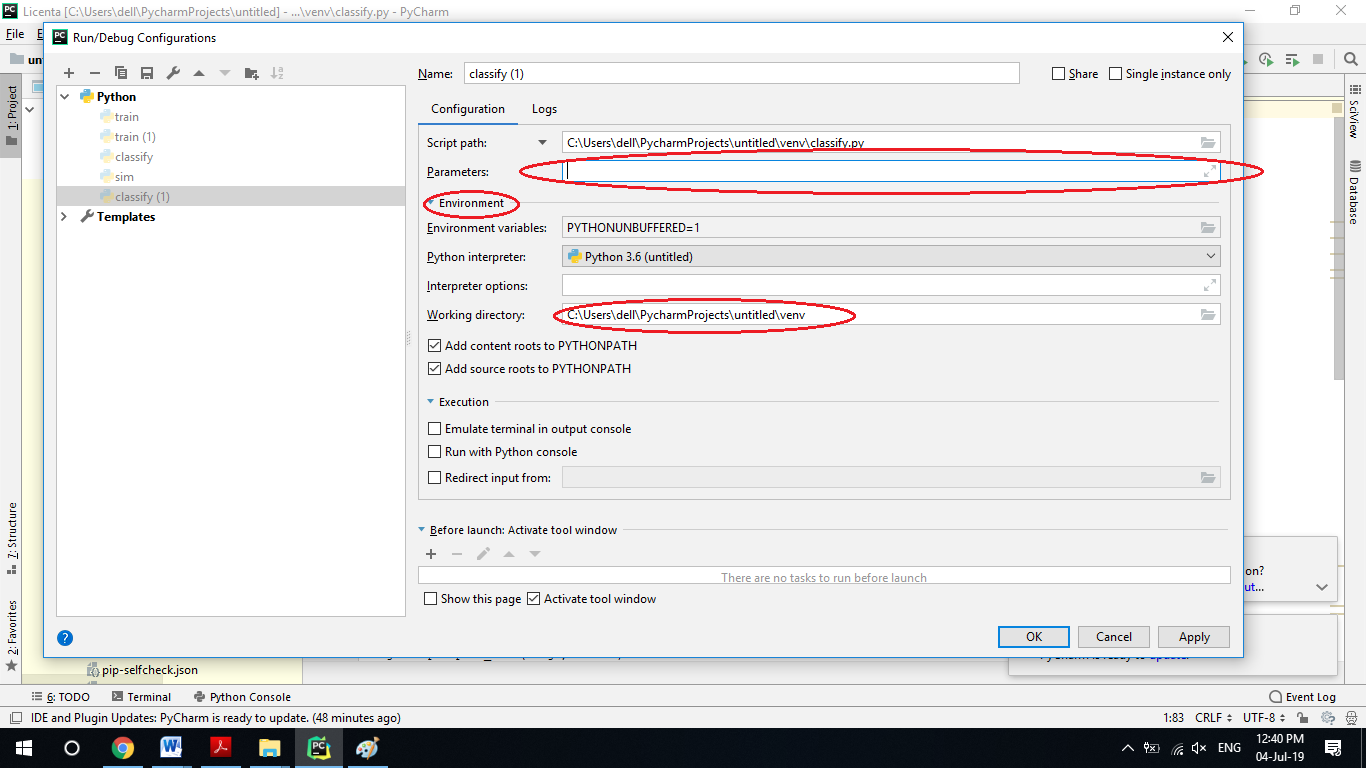
\includegraphics[width=15cm, height=9cm]{img/data/imagerun3.png}
	\caption[]
	{Introduce the correct arguments in the white space highlighted. Also, pay attention to the environment settings, because a lot of errors can happen by incorrectly specifying the variables there.}
	\label{fig:imagerun3}
\end{figure}

\begin{figure}[h!]
	\centering
	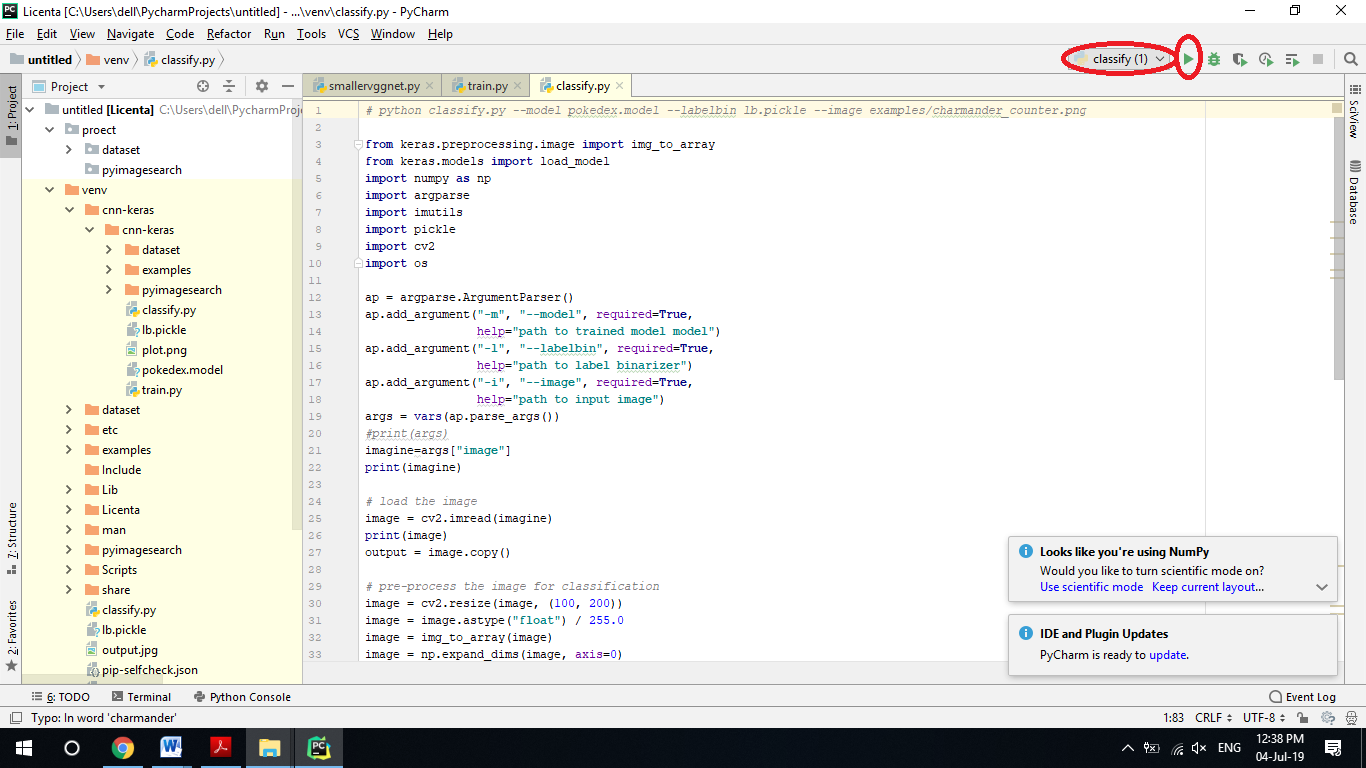
\includegraphics[width=15cm, height=9cm]{img/data/imagerun4.png}
	\caption[]
	{After verifying the arguments and parameters, one can run the training or classifying code by pressing the highlighted button. Also, pay attention to the highlighted name, next to the button. This specified the program that was compiled and will be run next.}
	\label{fig:imagerun4}
\end{figure}


\chapter{Conclusions}
\label{ch:conclusions}


After the concept was proven viable and the implementation yielded satisfactory results one can conclude the following aspects:
\begin{enumerate}
\item There is a need to study methods of object detection and image recognition involving deep learning processes, as well as more classical methods like haar features.
\item There is a need to study the realm of convolutional neural networks and their architectures
\item There is a need to implement the whole system in Python, taking into consideration hardware constraints and also, compared two different loss functions for binary classifications
\item The testing and validation process returned the almost-optimal solution for my system, which in the real world yielded satisfactory performances, which also comply with the initial requirements of the contractor
\end{enumerate}

Moreover, in book deep learning page 20. In \cite{book-deeplearning}, Yann Goodfellow mentiones that: "as of 2016, there exists an unofficial rule of thumb that a supervised deep learning classification algorithm will usually yield good enough performance with around 5000 labeled examples per category and will match or surpass human performance when trained with a dataset containing at least 10 million labeled examples. Working successfully with datasets smaller than this is an important research area and it needs more work, focusing especially on how we can take advantage of large quantities of unlabeled examples with unsupervised or semi-supervised learning". This statement shall be mentioned, when factoring in the fact that my dataset only had 1200 digital input images. Furthermore, at page 21 in \cite{book-deeplearning} the authors state that increasing model sizes is another key reason why neural networks are so successful today after having little success during the history of the \nth{20} century. It is possible because we have the computational resources to test and train much larger models today. One of the early statements of the connectionism movement is that animals become intelligent when many of their neurons work together. It results that one neuron or a small amount of neurons are not particularly useful for classifying problems, as well as any AI-based solution.\par


In order to develop this convolutional neural network-based defect detection proof-of-concept prototype, I started out by contouring the following targets and the following tasks:

\begin{enumerate}
    \item Literature research and studying relatied work in the domain of manufacturing.
    \item Literature research and studying related work in the domain of deep learning and convolutional neural networks
    \item Literature research and studying related work in the domain of image recognition and object detection
    \item Design and implementing a solution based on convolutional neural networks for defect detection in the specified manufacturing process
    \item Testing the proof-of-concept solution and analyzing the results
    \item Outlying the potential improvements and the implementation methods of the CNN-solution in the real world manufacturing process
\end{enumerate}

Every single sub-task was analyzed and the relationship between the sub-tasks was studied because in the beginning they were treated individually and after that they were combined, yield the aforementioned solution. Moreover, the prototype is complex because I tried to encompass every information learned along the way and to not cut out any single important mention in the domain. The deep convolutional neural network model is derived from the VGGNet architecture\cite{article-vgg} and was modified in order to be implementable on the available hardware. Once it was constructed and implemented, a training and testing strategy was needed, in order to find the optimal parameter and layer tweaking. Optimal parameters and layers configuration means that the whole system returns the smaller error rate possible.


\subsubsection{Result analysis}
First of all, the metrics of interest for the contractor OKOS Solution are: accuracy and mean classification time. In order to obtain the results, I needed to make sure that there is a compatible and good enough infrastructure in order to train and test the neural network algorithm. As mentioned in chapter 3, real world factory data was used in order to train the classifier. Based on the results obtained from the classification of the digital images fed as input, the defect detection algorithm returned a mean accuracy of around 80\% when using the binary cross entropy cost function and around 60\% when using the sparse categorical cross entropy cost function. The training time for the first model that used binary cross entropy was 6 hours, while the training time for the second one was around 4. One can derive the fact that it doesn`t justify using sparse categorical cross entropy, even if it reduces training time, the training time is not of interest for the contractor. The model will be trained on a computing station and then deployed into the manufacturing process. The mean classification time for newly acquired samples is around 10 seconds. It shall be again mentioned the fact that our interest is in newly acquired images, not in the test or training set. Also it is viable to assume the fact that in the factory environment, this algorithm shall be deployed on a micro-controller or a compute on the edge stick. Judging by the fact that these have hardware and computing constraints, the fact that a more general and computationally cheap solution was discussed seems to be a bonus. A big remark should be made here, because this is a solution developed in order to test the viability of a neural network solution for this vision-based task, so the development time and effort is and was not at great levels. Neither was the financial backup of the industry partner that requested this research. So it is safe to assume that a defect detection algorithm`s accuracy and classification time could easily converge to the state-of-the-art detection algorithm`s accuracies of around 95 to 99\%\cite{book-deeplearning}\cite{article-lecun}.\par


To improve the performances of a neural network one shall consider: increasing the model size over time, this is possible due to the increased availability of faster CPUs and GPUs, faster networking connections and better software infrastructure for distributed computing. As mentioned in \cite{book-deeplearning}, this trend of increased computing power is consensually expected to continue. It result that increasing the size and depth of a neural network model, is for now a viable solution(and for the next few decades).\par

The contractor OKOS Solutions did not provide us a clear cut performance measure of a human operator, but we can approximate it by looking at the average object detection accuracy, in digital images, of a human and than factor in working hours, different shifts of workers and the stamina of the human eye. In the paper \cite{article-studyhumandeep, article-studyhumandeep2} the authors state the fact that an average human has a mean detection accuracy of around 90\%. Additionally, in both it is mentioned the fact that usually deep neural systems are more sensible to perturbation and noise than humans. While a specific classification time was not mentioned, one can safely assume that at least 30 seconds would be needed for a human operator to analyze the whole image and than to make a decision. By factoring in these findings, in the following table, a side-by-side comparison of the neural network defect detection algorithm and the fictional average human operator is made:
\begin{table}[h!]
\centering
\begin{tabular}{ |p{3cm}||p{3cm}|p{3cm}| }
 \hline
 \multicolumn{3}{|c|}{\textbf{Human vs. machine comparison}} \\
 \hline
 \textbf{Name} & \textbf{Mean accuracy} & \textbf{Mean classification time} \\
 \hline
 Human operator & 90\% & >30 sec\\
 \hline
 CNN algorithm & 80\%(pathway to 95-99\%) & 10 sec\\
 \hline
\end{tabular}
\caption{Performance metrics.}
\end{table}
\par
The main conclusion from this side-by-side comparison is the fact that, the proof-of-concept algorithm is at least three times faster than an average human operator, while having comparable accuracy over new samples. Additionally, binary cross entropy is a way better cost function for defect detection than sparse categorical cross entropy. Furthermore, the pathway for an algorithm that can classify in less than 10 seconds and has a mean accuracy greater than 95\% was demonstrated.\par

Another important aspect that needs to be mentioned here is that at this project contracted by OKOS Solutions Ltd. from the USA, I worked together with a team other three colleagues, hence some of the similarities in the theoretical background and introduction. But every student chose his own approach, a different architecture and a different implementation: some chose Matlab, some Python. Still, a comparison need to be made in order to compare different solutions and different approaches as it can serve as a starting point for further research. The performance metrics are written in the table \ref{tab:toti} below. \textbf{Remark:} computation times differ because of architecture, but most importantly they differ because of the different hardware setups we had available.

\begin{table}[H]
\label{tab:toti}
 \begin{tabular}{|c |c| c | c| c| c| c|} 
 \hline
  & Tr data &  Test data & Layers & Acc & Comp time & Defects detected\\ 
 \hline
 Matlab(custom) & 25000 & 3970 & 18 & 99.64\% & 99.06\% & 0.5 \\ 
 \hline
 Matlab(custom) & 7800 & 1003 & 28 & 96.35\% & 96.35\% & 8.53 \\
  \hline
 Python AlexNet & 30700 & 4500 & 11 & 67\% & 99.8\% & 1 \\ 
 \hline
 Python VGGNet & 1000 & 200 & 5 & 80\% & 77\% & 10 \\
 \hline
 \end{tabular}
\caption{Performance metrics obtained. Robustness not taken into consideration. Ideal cases.}
\end{table}
\par



\subsubsection{Further developments}
By analyzing the obtained results and tracing the development time, it can be concluded that it is viable for such a type of solution in the industry for the specified process. Moreover, a path for yielding a generalized framework for solutions for vision-based tasks is demonstrated and contoured. In order to enhance the performance of the algorithm and in order to improve the portability, several changes and incremental improvements are needed. They are:

\begin{enumerate}
    \item It shall be first mentioned that a better hardware setup would greatly improve performances: use a faster and larger GPU with more memory and a faster CPU.
    \item With a new GPU, also new versions of the CUDA Toolkit can be used, which again improves the performances
    \item To integrate the developed prototype into the manufacturing process present at OKOS Solutions or a similar hardware setup in order to test the algorithm in a real world environment.
    \item Enhancing the algorithm performances, by using a larger training data set.
    \item Improving the accuracy by using a FASTER R-CNN very deep network architecture, because this type of neural network needs only 0.1-1 second per image, but tops other models in accuracy (which is our concern).
    \item Obtain a generalized network model that applies for all vision-based tasks that resemble the one studied, in order to be able to quickly adapt it to detect other defects.
    \item Obtain a generalized network model that applies for all vision-based tasks that resemble the one studied, in order to be able to quickly adapt it to detect other defects.
    \item Implement a dedicated user interface.
\end{enumerate}



\begin{thebibliography}{1}
%1
\bibitem{article-industrial}
J. Kapás, "Industrial revolutions and the evolution of the firm's organization: an historical perspective", 2008, Journal of Innovation Economics.
%2
\bibitem{article-aiemplo}
A. Sandybayev, "Artificial Intelligence: Are We All Going to Be Unemployed?," 2018 Fifth HCT Information Technology Trends (ITT), Dubai, United Arab Emirates, 2018, pp. 23-27.
%3
\bibitem{article-imagenet}
I. Sutskever, G.E. Hinton, A. Krizhevsky, "ImageNet classification with deep convolutional neural networks," in NIPS, vol. 1, 2012, pp. 1106-1114.
%4
\bibitem{article-vgg}
K. Simonyan, A. Zisserman, "Very Deep Convolutional Networks For Large-Scale Image Recognition," in ICLR, 2015.
%5
\bibitem{book-deeplearning}
Y. Bengio, A. Courville, I. Goodfellow, Deep Learning.: MIT Press, 2016, pp. 12-26.
%6
\bibitem{article-acusticmicro1}
T. M. Moore, R. McKenna and S. J. Kelsall, "Correlation of surface mount plastic package reliability testing to nondestructive inspection by scanning acoustic microscopy," 29th Annual Proceedings Reliability Physics 1991, Las Vegas, NV, USA, 1991, pp. 160-166.
%7
\bibitem{article-acusticmicro2}
S. D. Kent, S. J. Lockwood and H. Lee, "High resolution tomographic acoustic microscopy," Conference Record of The Twenty-Ninth Asilomar Conference on Signals, Systems and Computers, Pacific Grove, CA, USA, 1995, pp. 1051-1055 vol.2.
%8
\bibitem{article-acusticmicro3}
R. Shriram, J.E. Semmens, L. Kessler, "High-frequency acoustic microscopy studies of buried interfaces in silicon", Proceedings - Electronic Components and Technology Conference. 2006. 4 pp.
%9
\bibitem{article-manufef}
S. Ford, M. Despeisse, "Additive manufacturing and sustainability: an exploratory study of the advantages and challenges", Journal of Cleaner Production, Volume 137, pp. 1573-1587, 2016.
%10
\bibitem{book-historymanu2}
C. Roser, "Faster, Better, Cheaper in the History of Manufacturing: From the Stone Age to Lean Manufacturing and Beyond", Productivity Press, 1 edition, 2016.
%11
\bibitem{book-historymanu}
J. B. Freeman, "Behemoth: A History of the Factory and the Making of the Modern World", W. W. Norton \& Company, 1st edition, 2018.
%12
\bibitem{article-computervision}
T. Morris, "Computer Vision and Image Processing", Red Globe Press, 2004.
%13
\bibitem{article-cvapp}
R. Szeliski, "Computer Vision: Algorithms and Applications", Springer, 2010.
%14
\bibitem{article-cvhistory}
H. Grabner, C.Beleznai, "History of Computer Vision", OCG Journal, 2008, 3. 28-29. 
%15
\bibitem{article-boden}
M. A. Boden, "Mind as Machine: A History of Cognitive Science", 2006.
%16
\bibitem{article-snake}
M. Kass, A. Witkin, D. Terzopoulos, "Snakes: Active contour models" International Journal of Computer Vision, 1988.
%17
\bibitem{article-grimson}
W. E. L. Grimson, "Computational Experiments with a Feature Based Stereo Algorithm," in IEEE Transactions on Pattern Analysis and Machine Intelligence, vol. PAMI-7, no. 1, pp. 17-34, 1985.
%18
\bibitem{article-longuet}
H. C. Longuet-Higgins, "A computer algorithm for reconstructing a scene from two projections", Nature, vol. 293, pp. 133–135, 1981. 
%19
\bibitem{book-marr}
D. Marr, "Vision: A Computational Investigation into the Human Representation
and Processing of Visual Information", W. H. Freeman, San Francisco, 1982.
%20
\bibitem{article-violajones}
P. Viola, M.J. Jones, "Robust Real-Time Face Detection", in International Journal of Computer Vision, 57: 137, 2001.
%21
\bibitem{article-faceann}
H. Jiang, E. Learned-Miller, "Face Detection with the Faster R-CNN", 12th IEEE International Conference on Automatic Face \& Gesture Recognition, Washington, DC, pp. 650-657, 2017.7
%22
\bibitem{article-violaresult}
S. Liao, A. K. Jain and S. Z. Li, "A Fast and Accurate Unconstrained Face Detector," in IEEE Transactions on Pattern Analysis and Machine Intelligence, vol. 38, no. 2, pp. 211-223, 1 Feb. 2016.
%23
\bibitem{article-studyhumandeep}
S. Dodge, L. Karam, "A Study and Comparison of Human and Deep Learning Recognition Performance
Under Visual Distortions", cs.CV, 2017.
%24
\bibitem{article-lecungen}
Y. LeCun, "Deep learning and convolutional networks," 2015 IEEE Hot Chips 27 Symposium (HCS), Cupertino, CA, 2015, pp. 1-95.
%25
\bibitem{article-lecunhistory}
Y. LeCun, "1.1 Deep Learning Hardware: Past, Present, and Future," 2019 IEEE International Solid- State Circuits Conference - (ISSCC), San Francisco, CA, USA, 2019, pp. 12-19.
%26
\bibitem{article-peddet}
P. Sermanet, K. Kavukcuoglu, S. Chintala and Y. Lecun, "Pedestrian Detection with Unsupervised Multi-stage Feature Learning," 2013 IEEE Conference on Computer Vision and Pattern Recognition, Portland, OR, 2013, pp. 3626-3633.
%27
\bibitem{article-objlocaliz}
J. Tompson, R. Goroshin, A. Jain, Y. LeCun and C. Bregler, "Efficient object localization using Convolutional Networks," 2015 IEEE Conference on Computer Vision and Pattern Recognition (CVPR), Boston, MA, 2015, pp. 648-656.
%28
\bibitem{article-ciresantraffic}
D. Cireşan, U. Meier, J. Masci and J. Schmidhuber, "A committee of neural networks for traffic sign classification," The 2011 International Joint Conference on Neural Networks, San Jose, CA, 2011, pp. 1918-1921.
%29
\bibitem{article-detandsegmmanu}
M. Ferguson, R. Ak, Y. Tina Lee, H.K. Law, "Detection and Segmentation of Manufacturing Defects with Convolutional Neural Networks and Transfer Learning", 2, 2018.
%30
\bibitem{article-autonomous1}
M. V. Rajasekhar and A. K. Jaswal, "Autonomous vehicles: The future of automobiles," 2015 IEEE International Transportation Electrification Conference (ITEC), Chennai, pp. 1-6, 2015.
%31
\bibitem{article-trafficsigndet}
J. Serrat, A.M. López, R. Baldrich, D. Gerónimo, "Traffic Sign Recognition for Computer Vision Project-Based Learning," in IEEE Transactions on Education, vol. 56, no. 3, 2013, pp. 364-371.
%32
\bibitem{article-lecuntraffic}
P. Sermanet and Y. LeCun, "Traffic sign recognition with multi-scale Convolutional Networks," The 2011 International Joint Conference on Neural Networks, San Jose, CA, 2011, pp. 2809-2813.
%33
\bibitem{article-ciresannumere}
D. Ciresan, D. Pescaru, "Off-line recognition of handwritten numeral strings composed from two-digits partially overlapped using Convolutional Neural Networks," 2008 4th International Conference on Intelligent Computer Communication and Processing, Cluj-Napoca, 2008, pp. 53-60.
%34
\bibitem{article-lecunhousenr}
P. Sermanet, S. Chintala and Y. LeCun, "Convolutional neural networks applied to house numbers digit classification," Proceedings of the 21st International Conference on Pattern Recognition (ICPR2012), Tsukuba, 2012, pp. 3288-3291.
%35
\bibitem{article-lecun}
B. Boser, J.S. Denker, D. Henderson, R.E. Howard, W. Hubbard, L.D. Jackel, Y. LeCun, "Backpropagation applied to handwritten zip code recognition," in Neural Computation, Volume 1, Issue 4, 1989, pp. 541-551.
%36
\bibitem{article-industry4}
C. Klingenberg, "Industry 4.0: what makes it a revolution?", EurOMA, 2017.
%37
\bibitem{article-agingpop}
M. Chand, R. Tung, "The Aging of the World's Population and Its Effects on Global Business. Academy of Management Perspectives", 2014.
%38
\bibitem{article-fabrics}
A. Kumar, "Computer Vision-based Fabric Defect Detection: A Survey," in IEEE Transactions on Industrial Electronics ( Volume: 55 , Issue: 1 , Jan. 2008 ), 2008, pp. 348 - 363.
%39
\bibitem{article-metalsurfacelinguridet}
Z. Li, J. Zhang, T. Zhuang and Q. Wang, "Metal surface defect detection based on MATLAB," 2018 IEEE 3rd Advanced Information Technology, Electronic and Automation Control Conference (IAEAC), Chongqing, 2018, pp. 2365-2371.
%40
\bibitem{article-mettalicsurfacedet}
X. Tao, D. Zhang, W. Ma, X. Liu, D. Xu, "Automatic Metallic Surface Defect Detection and Recognition with Convolutional Neural Networks", 2018, Applied Sciences, 8, 1575.
%41
\bibitem{article-wheelhubdet}
K. Han, M. Sun, X. Zhou, G. Zhang, H. Dang and Z. Liu, "A new method in wheel hub surface defect detection: Object detection algorithm based on deep learning," 2017 International Conference on Advanced Mechatronic Systems (ICAMechS), Xiamen, 2017, pp. 335-338.
%42
\bibitem{article-tirexraydet}
Q. Zhu, X. Ai, "The Defect Detection Algorithm for Tire X-Ray Images Based on Deep Learning," 2018 IEEE 3rd International Conference on Image, Vision and Computing (ICIVC), Chongqing, 2018, pp. 138-142.
%43
\bibitem{article-ciresan}
U. Meier, J. Masci, L.M. Gambardella, D.C. Ciresan, "Flexible, High Performance Convolutional Neural Networks for Image Classification," in International Joint Conference on Artificial Intelligence IJCAI-2011, 2011, pp. 1237-1242.
%44
\bibitem{article-understandingcnn}
R. Fergus, M.D. Zeiler, "Visualizing and Understanding Convolutional Neural Networks," in ECCV 2014, Part I, LNCS 8689. 8689. 2013.
%45
\bibitem{article-lecuncnn}
Y. LeCun, K. Kavukcuoglu and C. Farabet, "Convolutional networks and applications in vision," Proceedings of 2010 IEEE International Symposium on Circuits and Systems, Paris, 2010, pp. 253-256.
%46
\bibitem{article-rcnn}
R. Girshick, J. Donahue, T. Darrell and J. Malik, "Rich Feature Hierarchies for Accurate Object Detection and Semantic Segmentation," 2014 IEEE Conference on Computer Vision and Pattern Recognition, Columbus, OH, 2014, pp. 580-587.
%47
\bibitem{article-fastrcnn}
R. Girshick, "Fast R-CNN", in ICCV Proceedings'15 of the 2015 IEEE International Conference on Computer Vision, pp. 1440-1448, 2015. 
%48
\bibitem{article-fasterrcnn}
S. Ren, K. He, R. Girshick, J. Sun, "Faster R-CNN: Towards Real-Time Object
Detection with Region Proposal Networks", in IEEE Transactions on Pattern Analysis and Machine Intelligence, 2016.
%49
\bibitem{article-yolo}
J. Redmon, S. Divvala, R. Girshick, A. Farhadi, "You Only Look Once: Unified, Real-Time Object Detection". 779-788. 2016. 10.1109/CVPR.2016.91.
%50
\bibitem{article-maxpooling}
Zhou and Chellappa, "Computation of optical flow using a neural network," IEEE 1988 International Conference on Neural Networks, San Diego, CA, USA, 1988, pp. 71-78 vol.2.
%51
\bibitem{article-adam}
D. Kingma, J. Ba, "Adam: A Method for Stochastic Optimization", International Conference on Learning Representations, 2014.
%52
\bibitem{article-studyhumandeep2}
R. Geirhos, D. H. J. Janssen, H. H. Schütt, J. Rauber, M, Bethge, F. A. Wichmann, "Comparing deep neural networks against humans:
object recognition when the signal gets weaker", 2017.

\end{thebibliography}
\title{Appendix}
\chapter{Appendix}

\end{document}
